%!TeX program = xelatex
\documentclass[13.5pt,hyperref,a4paper,UTF8]{ctexart}
\usepackage{UESTCpapers}
\usepackage{threeparttable}
\usepackage{float}
\usepackage[figuresleft]{rotating}
\usepackage{longtable}
\usepackage{makecell}
\xeCJKsetup{CJKmath=true} 

\renewcommand{\floatpagefraction}{.9}

\linespread{1.5}
%%-------------------------------正文开始---------------------------%%
\begin{document}


%%-----------------------封面--------------------%%
\cover

\thispagestyle{empty} % 首页不显示页码
%%------------------摘要-------------%%
\newpage
\begin{abstract}
~\\
~\\
~\\
~\\
%
\indent 本文针对金融领域信用贷款的审核、评估、预测这一复杂难题,运用计量经济学方法进行了深入研究。

首先,本文对现有信贷模型的理论基础和文献内容进行了研讨分析,以初步了解影响还款行为的潜在因素。随后,我们对某公司的两个公开数据集的基本数据特征、分布特征、相关系数进行了简要分析。

在此基础上,我们分别针对这两个数据集构建了还款能力模型和坏账金额预测模型。

在还款能力模型中,我们考虑了多个影响因素,如申请人的年龄、婚姻状况、子女个数、教育程度和所在城市 GDP 评级等。我们采用 Logit 模型分析申请人的还款能力,以帮助贷款机构在审核贷款申请时更准确地评估申请人的信用风险。

坏账金额预测模型则旨在预测贷款违约时的坏账金额。通过分析违约贷款的债务资产比、信用评级、年龄等因素,我们拟合出了一个线性回归模型。并对模型进行了多重共线性、模型设定、序列相关性、异方差的检验及修正。

本文的研究结论具有一定的理论和实践意义。首先,还款能力模型为贷款机构提供了一个有效的评估申请人信用风险的工具,有助于降低贷款违约风险。其次,坏账金额预测模型为贷款机构在面临坏账时提供了预警和应对策略,有助于减轻贷款损失。此外,这两个模型还可为其他金融机构和企业在信贷审核、评估和预测方面提供借鉴和参考。

总之,本文通过深入研究信用贷款的审核、评估、预测问题,为金融领域提供了一种有效的信用风险管理手段。
%
~\\
~\\
~\\
% 关键词
\textbf{关键词}:信用贷款, 还款预测, 坏账估计, Logit模型, 线性回归 
\addcontentsline{toc}{section}{摘要}\tolerance=100 %将摘要放进目录 
\end{abstract}
\thispagestyle{empty} % 首页不显示页码

%%--------------------------目录页------------------------%%
\newpage
\addcontentsline{toc}{section}{目录}\tolerance=100 %将摘要放进目录 
\tableofcontents




%%------------------------正文页从这里开始-------------------%
\newpage

%%可选择这里也放一个标题
%\begin{center}
%    \title{ \Huge \textbf{{标题}}}
%\end{center}

%\section{定理环境}
%\begin{Theorem}
%\end{Theorem}
%
%\begin{Lemma}
%\end{Lemma}
%
%\begin{Corollary}
%\end{Corollary}
%
%\begin{Proposition}
%\end{Proposition}
%
%\begin{Definition}
%\end{Definition}
%
%\begin{Example}
%\end{Example}
%
%\begin{proof}
%\end{proof}

\section{选题背景与调研}
\indent  本节将首先阐述本题目的现实背景,从社会现象分析课题的现实意义。接着,通过文献调研,总结提出了初步的研究见解。此外,本节还将对一些基础理论进行详细说明,为后续的实证研究奠定理论基础。
\subsection{选题背景与社会现状}
\indent 近年来,我国经济持续高速发展,人民生活水平不断提高,消费观念发生了深刻变化。越来越多的人开始倾向于"提前消费",即将未来的财富提前到现在消费,这已成为一种新的消费趋势。

这种消费观念的转变推动了金融信贷市场的快速发展。用未来的钱来满足现在的需求,金融信贷市场也得以日益强大。阿里的花呗、蚂蚁积分、人人贷等金融网贷平台凭借高效便捷的服务迅速吸引力大量的群众。中国人民银行发布数据显示,2021年末,金融机构人民币各项贷款余额192.69万亿元,同比增长11.6\%;全年人民币贷款增加19.95万亿元,同比多增3150亿元。\cite{loanStatisticCH1}

贷款数量的增加必然会带来金融风险的增加,由于信息不对称导致金融网络借贷信用风险也日益凸显。一些信用良好且还款能力强的客户往往也因此被拒之门外。同时每年都有众多金融信贷机构因为资金链断裂、违约、骗贷等原因而倒闭停业,其数量已高达上千家。因此,如何回答金融机构该不该借钱?如何有效管理贷款人情况,做出准确风险判断?当预期贷款人已经不能正常还款,如何准确预估坏账的金额大小?这一系列问题,成为了亟需解决的问题。

基于以上现象,我们小组决定对以下两个主要问题进行探究:

\quad \textbf{(a)} \quad \underline{判断借款人是否有能力还款的可能影响因素有哪些?}

\quad \textbf{(b)} \quad  \underline{如何估计某一贷款的坏账金额?}


\subsection{文献调研与理论基础}

为了初步探究逾期行为与坏账大小的影响因素,小组进行了相关文献调查并进行了理论研究。

一些国外的研究认为影响贷款逾期和坏账的因素包括贷款政策、信誉衡量标准、绩效指标、宏观经济环境和银行特定因素等。Ikram 等人 (2016) 以及 Nikolopoulos 和 Tsalas (2017) 对不良贷款的影响因素进行了讨论,提到了经济增长、通货膨胀、房地产价格、利率和汇率等宏观经济因素,以及银行对借款人或抵押品的评估、法律和监管环境的影响 \cite{1ikram2016determinants,2nikolopoulos2017non}。Fennee Chong (2021) 对影响贷款拖欠的因素进行了调查,发现借款人与贷款人的距离、抵押品、教育水平和每月预算具有显著影响,但是收入和性别则没有显著影响 \cite{3chong2021loan}。Matteo Foglia (2022) 调查了宏观经济因素对意大利银行系统不良贷款的影响,发现生产总值和公共债务对不良贷款有负面影响,而失业率和国内信贷对减值贷款产生积极影响 \cite{4foglia2022non}。

国内关于信用贷款逾期行为影响因素的研究也十分广泛。在《互联网贷款个人信用风险影响因素研究综述》\cite{李焱文2020互联网贷款个人信用风险影响因素研究综述}中,作者将贷款逾期行为的主要因素简单分为三类。

一是如\textbf{借款人个体显著特征},如\textit{学历、年龄、婚姻},该类影响因素占主要成分。我们在文献《流量覆盖风险——网络小额信贷风险控制新思路》\cite{蔡闽2016流量覆盖风险——网络小额信贷风险控制新思路}中也找到了对这一观点的实证。其实证显示\textit{女性相比男性更谨慎信用风险更低、年龄较大的借款人违约率更低、受教育程度与违约率呈负相关、已婚人士比未婚和单身人士信用更优,婚姻稳定者违约率较低,收人较高的借款人拥有更低的违约率。}

二是\textbf{借款人关联特征},如\textit{家庭、资产、居住城市},该类影响因素对一个人的贷款信用高低有着一定的关联。根据文献《城市信用环境对个人贷款保证保险违约风险影响的研究》\cite{栾伊娜2020城市信用环境对个人贷款保证保险违约风险影响的研究}的调研显示,\textit{良好的城市信用环境,会降低违约风险}

三是\textbf{历史记录与贷款产品}特征,这类数据通常是由信贷机构基于对用户画像的评分和用户申请时填写,如\textit{历史违约次数、申请金额高低}。文献《P2P网贷借款人信用风险因素分析与对策》\cite{雷舰2019P2P网贷借款人信用风险因素分析与对策}谈到\textit{逾期次数与违约概率直接正相关,成功次数多者申请次数越多,违约比例越小,同时,违约较多发生在申请次数较少的新借款人中。}

在相关文献中,我们也看到了两个比较新颖的评判指标——\texttt{ltv}和\texttt{ita}。其相关计算公式如下。
\begin{equation}
\begin{split}
    ltv=\frac{loanAmount}{Asset}\\
    \\
    ita=\frac{income}{annAmount}\nonumber
\end{split}
\end{equation}

可以看到,\texttt{ltv}反映了借款人借款金额和拥有资产的比率,\texttt{ita}反映了借款人收入和每年还款金额的比例。这两个指标在信用贷款的评估中是一个被广泛使用的度量标准。例如,在文献《个人住房抵押贷款的市场风险研究》\cite{杨青2011个人住房抵押贷款的市场风险研究}显示\textit{LTV值越大,违约风险越大}。在这种情况下,若借款人违约,银行收回的资产可能无法弥补贷款损失,从而导致银行的风险暴露越大。此外,较高的 \texttt{ltv}值也可能意味着借款人负担过重,还款压力较大,进一步增加了违约的可能性。因此,银行和金融机构在审批贷款时,通常会密切关注\texttt{ltv} 值,对过高 \texttt{ltv} 值的贷款申请进行更严格的审核,以确保风险可控。

\texttt{ita}值则是衡量借款人收入偿还能力的重要指标。较高的 \texttt{ita} 值意味着借款人在还款过程中承担了较大的负担,可能会影响其生活质量并加大违约风险。银行在评估贷款申请时,会通过分析 \texttt{ita} 值来判断借款人的还款能力。若 \texttt{ita} 值过高,银行可能会认为借款人承受不了如此大的还款压力,从而拒绝贷款申请或采取更高的利率措施以降低风险。


\newpage
\section{数据收集与分析} 
本节重点阐述了数据集的来源,并对数据集进行了简洁的概述。同时,我们对数据集实施了初步的预处理工作。之后,将预处理后的数据导入到 Eviews 软件中,对其数据特征进行了分析。在这个过程中,我们初步探讨了数据的内在规律和联系,为后续的研究奠定了坚实的基础。
\subsection{数据来源与初步处理}
\subsubsection{数据集概述}
为了深入研究借款人还款能力的影响因素以及估算某一贷款的坏账金额,我们从 Kaggle 网站的大数据集中获取了两个较为有用的数据集信息。这两个数据集分别涵盖了各类借款人的信用记录和贷款情况,为我们提供了丰富的数据样本。通过对这些数据进行深入分析,我们期望能够发现借款人还款能力的关键影响因素,并为金融行业提供有效的风险防控措施。相关数据集概况如下:

\quad \textbf{I.} \quad \textbf{还款能力:贷款审批数据集}

第一个数据集包含了大量借款人的信用记录,包括借款人的基本信息、财务状况、资产情况等多个方面的数据。这个数据集为我们研究借款人还款能力的影响因素提供了丰富的数据支持。我们可以通过构建Logit模型,探究哪些因素是影响申请人还款的重要因素。数据集见参考文献\cite{database1CH2}

\quad \textbf{II.} \quad  \textbf{坏账金额:某信贷公司的两轮贷款业务中的坏账数据集 }

第二个数据集聚焦于贷款的违约情况,包含了贷款的坏账金额(违约损失)等关键指标。利用这个数据集,我们可以对不同情况的贷款申请进行坏账风险评估,并预测可能的坏账金额。这对于金融机构在审慎放贷、防范金融坏账风险方面具有重要的指导意义。数据集见参考文献\cite{databse2CH2}。

\subsubsection{数据预处理}
在将数据导入Eviews之前,我们需要进行一系列简单的处理,以便为后续的分析做好准备。

首先,我们需要剔除数据集中的异常值。以第二个数据集为例,其中的性别信息被分为三个变量,分别为“MALE”表示男性、“FEMALE”表示女性,以及“OTHER”表示其他。第三个变量“OTHER”的出现,是由于数据集在性别这一项的录入存在不足,部分用户并未填写性别信息。因此,我们需要将这些异常值排除在外。

其次,我们需要对数据集中的某些变量设置虚拟变量。以第一个数据集中的堆对城市评级为例,其评级由字符串“GOOD”,“NORMAL”和“BAD”表示。然而,Eviews 无法直接处理和标记这类字符串变量。为此,我们需要事先将这些变量转换为 1 和 0 的数值形式,设定两个虚拟变量“POOR”和“RICH”,分别标识该地区评级是否为“GOOD”、该地区评级是否为“BAD”。以便在后续的分析过程中能够顺利进行。

综上所述,在数据集处理过程中,我们需要进行两项主要操作:一是排除异常值,二是设置虚拟变量。这样,在完成这些基础工作之后,我们就可以继续进行下一步的数据分析了。

\subsection{特征解读与简要分析}
\subsubsection{数据集I:还款能力数据集}

我们将数据集I导入到Eviews软件中,进行初步的数据分布分析。
\begin{figure}[!htbp]
    \centering
    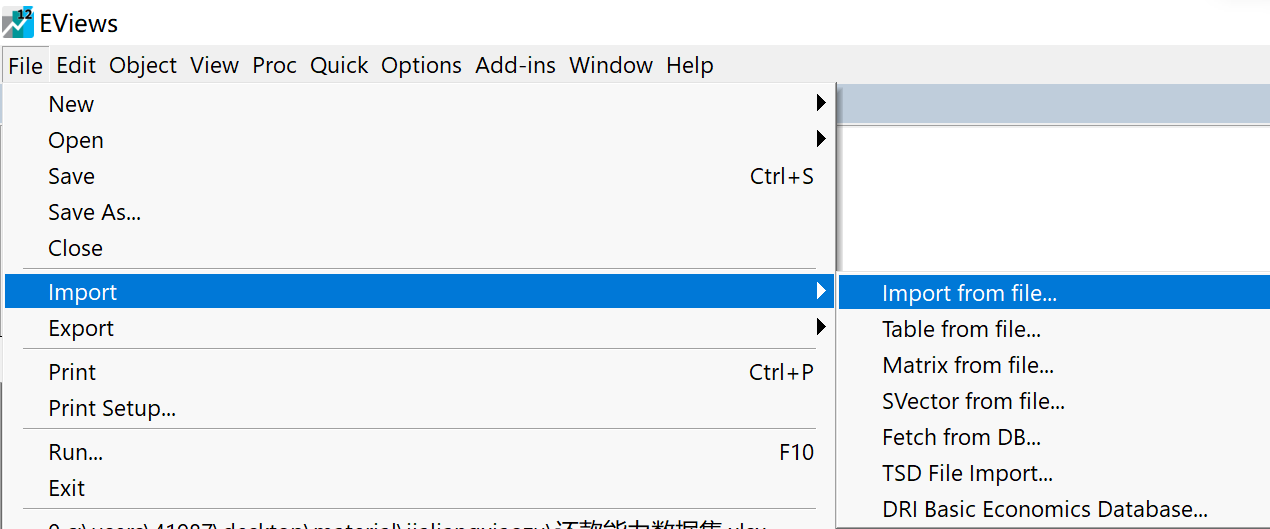
\includegraphics[width =.8\textwidth]{figures/2DATABASE/IMPORTDATABSE.png}
    \caption{导入数据到Eviews中}
    \label{导入数据到Eviews中}
\end{figure}

本数据集的全部变量的解释如表\ref{数据集I变量组成描述}所示:
\begin{table}[!htbp]
    \setlength{\belowcaptionskip}{0.2cm}
    \centering
    \caption{数据集I变量组成描述}
    \begin{threeparttable}
    \begin{tabular}{c  | p{5cm} |p{7cm}}
    \hline
        \textbf{变量名} & \textbf{解释} & \textbf{取值} \\
        \hline
        \texttt{target}  & 借款人是否存在还款困难\tnote{*}  &虚拟变量,是为1,不是则为0 \\
         \texttt{annamount}  & 借款人每年还款金额 &整数 \\
        \texttt{age}  & 借款人的年龄 & 整数 \\
        \texttt{income}  & 借款人的收入 & 整数 \\
        \texttt{gend}  & 借款人的性别 & 虚拟变量,男性为1,女性则为0 \\
        \texttt{family}  & 家庭人口数量 & 整数 \\
        \texttt{children}  & 抚养子女的数量 & 整数 \\
        \texttt{graduate} & 是否大学毕业 & 虚拟变量,是为1,不是则为0\\
        \texttt{marry}  & 当前是否已婚 & 虚拟变量,是为1,不是则为0 \\
        \texttt{car}  & 借款人是否拥有车辆 & 虚拟变量,是为1,不是则为0\\
        \texttt{house}  & 借款人是否拥有公寓或者住宅 & 虚拟变量,是为1,不是则为0\\
        \texttt{population}  & 借款人居住城市的人口数量 & 整数\\
        \texttt{rich}  & 借款人居住城市的GDP评级是否为优\tnote{**} & 虚拟变量,是为1,不是则为0\\
        \texttt{poverty}  & 借款人居住城市的GDP评级是否为差\tnote{**} & 虚拟变量,是为1,不是则为0\\
        \hline
    \end{tabular}
    \label{数据集I变量组成描述}
     \begin{tablenotes}
        \footnotesize
        \item[*] 相比“借款人是否最终还上款”,我们更关注借款人\textbf{在还款期间}是否存在还款困难的情况,\textbf{而不是只是最后的时间点}。所以变量的设定不是“借款人是否还清”,请注意。
        \item[**] 城市的评级分为“优”、“中”、“差”,以信贷机构给出的评级为准  %此处加入注释*信息

      \end{tablenotes}
    \end{threeparttable}
\end{table}

如图\ref{还款能力数据集变量情况}导入结果所示,数据集共含有27569个有效数据。值得说明的是,根据教材,在大样本下,极大似然估计量(Logit模型)仍有无偏性和最小方差性,因此在这里不必考虑大样本对显著性的影响。图\ref{整数字段分布}显示了整数字段(包括\texttt{age、annamount、children、family、income、population})的分布情况。可以看到,年龄字段分布最为均衡,年度还款金额和收入水平较为集中。借款人申请的贷款年金和收入水平差距不大。

\begin{figure}[H]
    \centering
    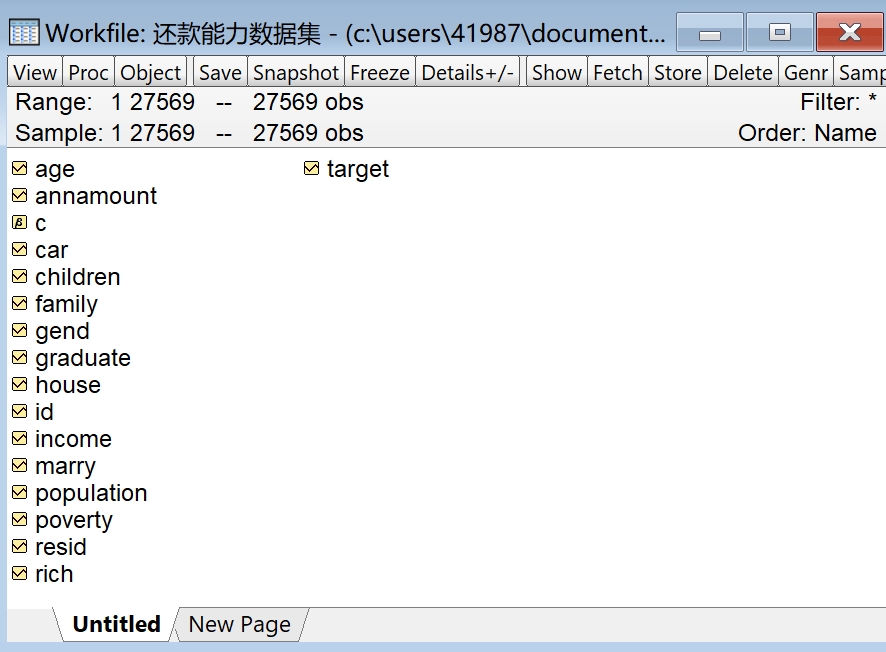
\includegraphics[width =.6\textwidth]{figures/2DATABASE/还款能力数据集变量情况.png}
    \caption{数据集I:还款能力数据集变量导入结果}
    \label{还款能力数据集变量情况}
\end{figure}

\begin{figure}[H]
    \centering
    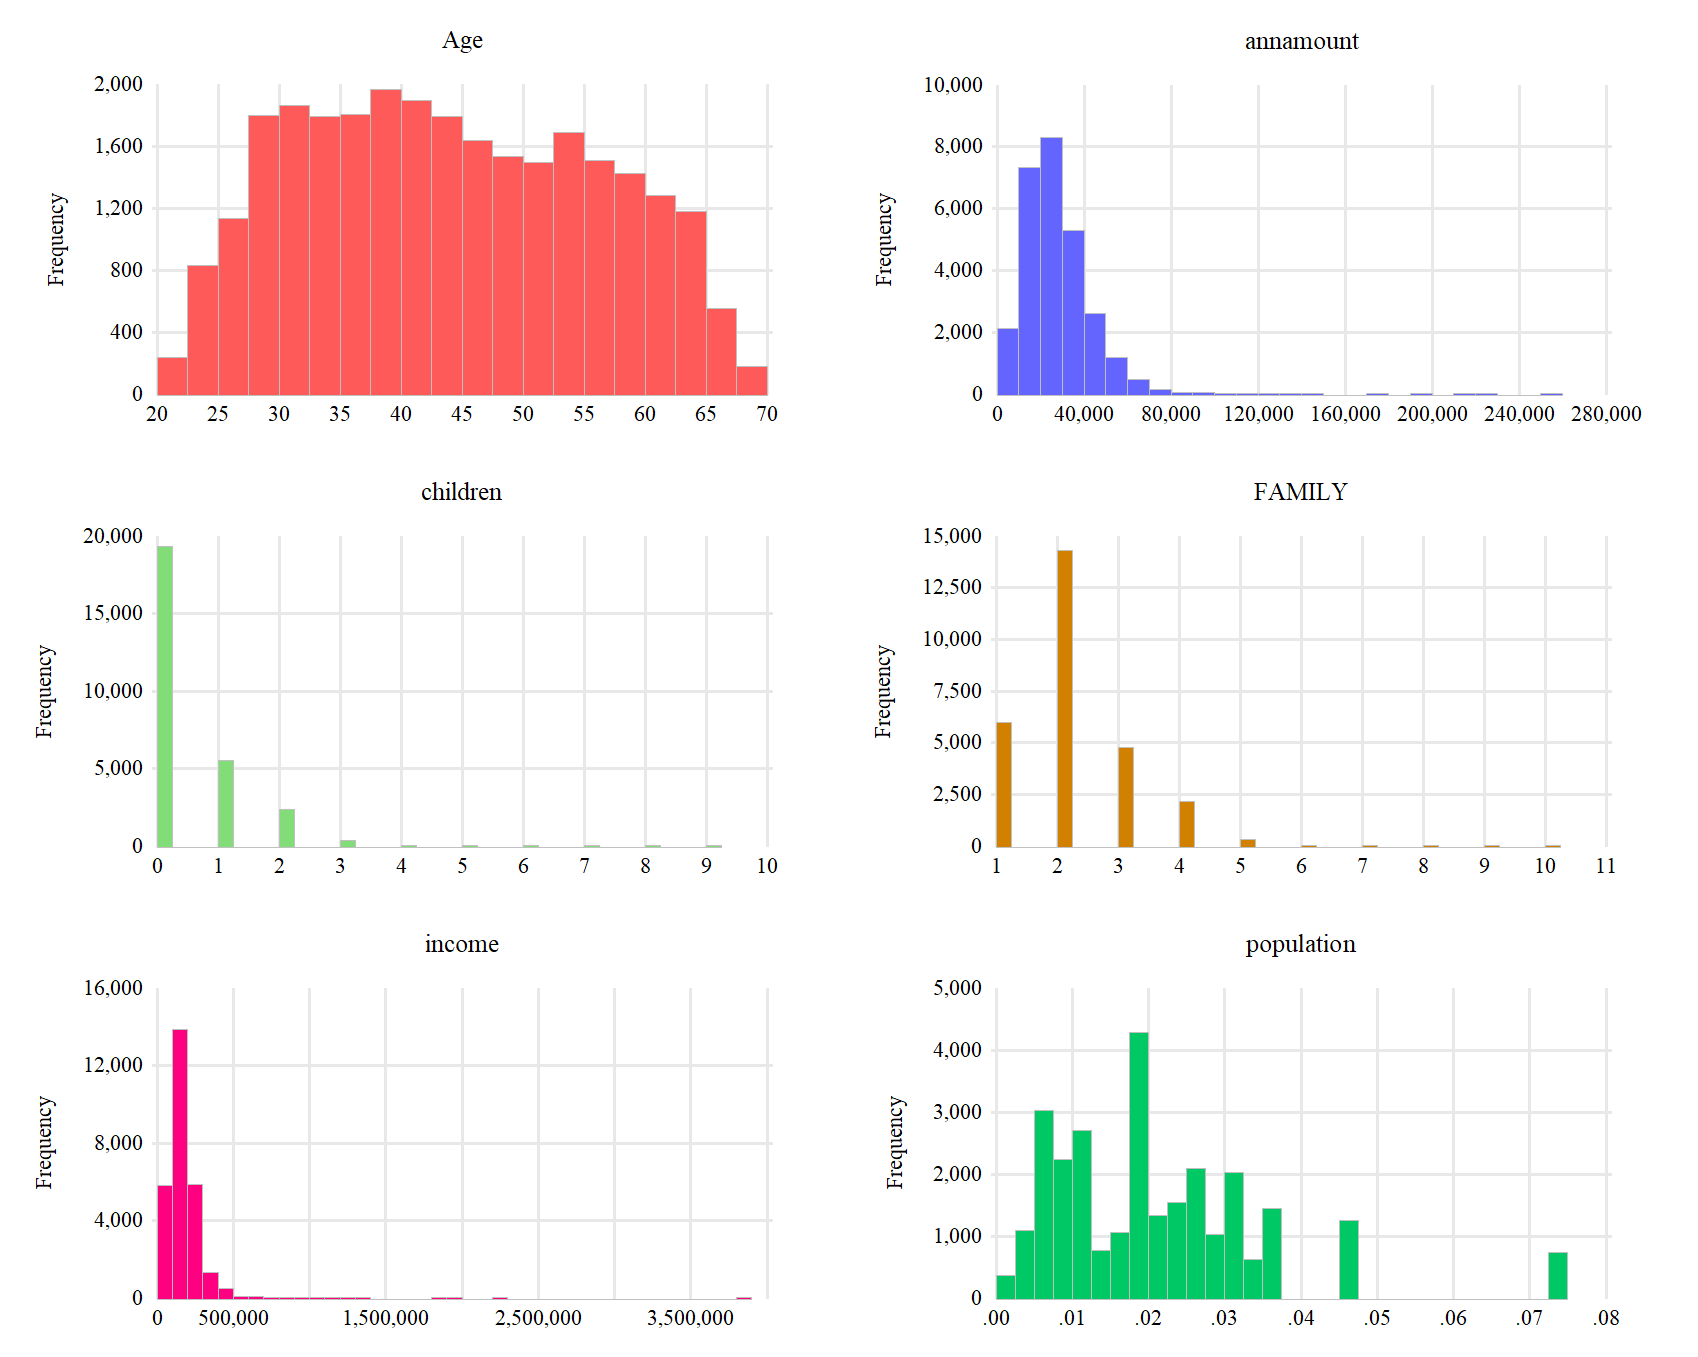
\includegraphics[width =.9\textwidth]{figures/2DATABASE/整数字段分布.png}
    \caption{数据集I:整数字段分布}
    \label{整数字段分布}
\end{figure}


\begin{figure}[H]
    \centering
    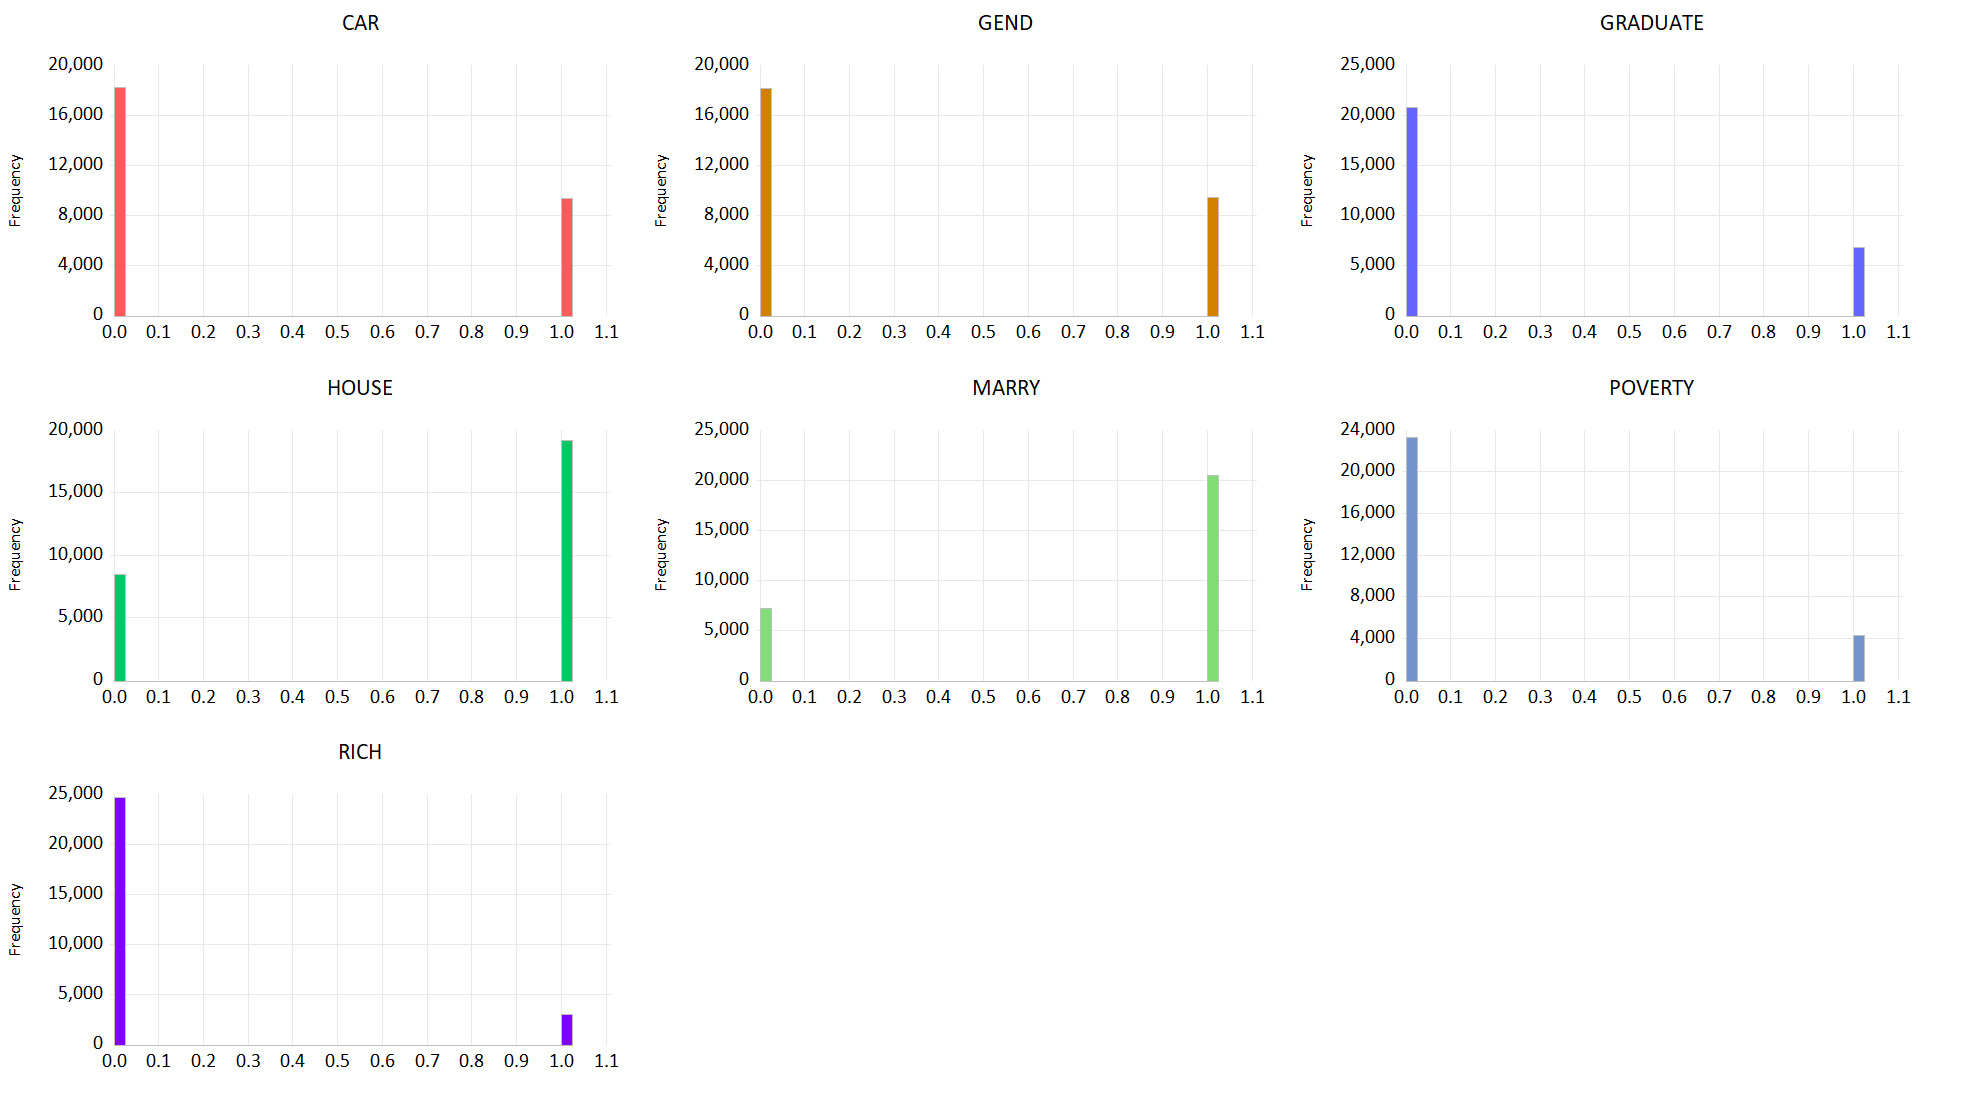
\includegraphics[width =1\textwidth]{figures/2DATABASE/数据集I虚拟变量字段分布.png}
    \caption{虚拟变量字段分布}
    \label{虚拟变量字段分布}
\end{figure}


\indent 图\ref{虚拟变量字段分布}展示了虚拟变量字段(包括\texttt{car、gend、graduate、house、marry、proverty、rich})的分布情况。可以看到,性别字段分布最为均衡,rich变量的分布较为集中。可能的原因是信贷机构评估的“好”的城市数量较少,我们在后续会结合\texttt{proverty}字段一同来对目标变量作回归分析。

综合来看,数据集数据分布均衡。下面对数据集特征作简要分析。

表\ref{整数数据样本描述特征}展示了数据集I中整数数据样本特征。例如,我们可以看到,数据集中平均年龄为43岁,借款样本中最高收入为258025.5,最低收入为2052.0,分布广泛。各个数据的均值、方差、标准差等均在正常范围以内,认为导入的数据正确无误。

表\ref{整数数据样本相关系数表(数据集1)}展示了数据集I中整数数据之间的的相关系数,可以看到,除\texttt{family}和\texttt{children}外,其他变量的相关系数均低于0.8。\texttt{family}和\texttt{children}都表征了样本数据家庭人口情况,因此其相关系数较大,在后续变量选取中,将纳入最好的一个。由于版面原因,我们没有办法展示虚拟变量之间的相关系数和数据描述,但是经过我们的实操,发现各个虚拟变量与其他变量的相关系数均小于0.8。

\begin{sidewaystable}[htp]
    \setlength{\belowcaptionskip}{0.2cm}
    \centering
    \caption{数据集II:整数数据样本特征}
    \begin{tabular}{|l|l|l|l|l|l|l|}
    \hline
        \textbf{ } & \textbf{AGE} & \textbf{ANNAMOUNT} & \textbf{CHILDREN} & \textbf{FAMILY} & \textbf{INCOME} & \textbf{POPULATION} \\ \hline
        \textbf{ Mean} &  43.92707 &  27177.27 &  0.416156 &  2.157858 &  168485.5 &  0.020786 \\ 
        \textbf{ Median} &  43.16438 &  24997.50 &  0.000000 &  2.000000 &  148500.0 &  0.018850 \\ 
        \textbf{ Maximum} &  68.99178 &  258025.5 &  9.000000 &  10.00000 &  3825000. &  0.072508 \\ 
        \textbf{ Minimum} &  21.04110 &  2052.000 &  0.000000 &  1.000000 &  25650.00 &  0.000533 \\ 
        \textbf{ Std. Dev.} &  11.94650 &  14662.61 &  0.722796 &  0.908802 &  98940.63 &  0.013777 \\ 
        \textbf{ Skewness} &  0.117600 &  1.816131 &  1.901573 &  0.959529 &  5.043504 &  1.478870 \\ 
        \textbf{ Kurtosis} &  1.951234 &  14.72883 &  7.599771 &  4.649344 &  100.0198 &  6.226274 \\ 
        \textbf{ } &   &   &   &   &   &   \\ 
        \textbf{ Jarque-Bera} &  1327.023 &  173177.9 &  40919.07 &  7355.318 &  10929496 &  22005.89 \\ 
        \textbf{ Probability} &  0.000000 &  0.000000 &  0.000000 &  0.000000 &  0.000000 &  0.000000 \\ 
        \textbf{ } &   &   &   &   &   &   \\ 
        \textbf{ Sum} &  1211025. &  7.49E+08 &  11473.00 &  59490.00 &  4.64E+09 &  573.0511 \\ 
        \textbf{ Sum Sq. Dev.} &  3934473. &  5.93E+12 &  14402.44 &  22769.00 &  2.70E+14 &  5.232924 \\ 
        \textbf{ } &   &   &   &   &   &   \\ 
        \textbf{ Observations} &  27569 &  27569 &  27569 &  27569 &  27569 &  27569 \\ \hline
    \end{tabular}
    \label{整数数据样本描述特征}
\end{sidewaystable}

\begin{sidewaystable}[htp]
    \setlength{\belowcaptionskip}{0.2cm}
    \centering
    \caption{数据集II:整数数据样本相关系数表}
    \begin{threeparttable}
    \begin{tabular}{|c|c|c|c|c|c|c|}
    \hline
        \textbf{ } & \textbf{AGE} & \textbf{ANNAMOUNT} & \textbf{CHILDREN} & \textbf{FAMILY} & \textbf{INCOME} & \textbf{POPULATION} \\ \hline
        \textbf{AGE} &  1.000000 & -0.008217 & -0.332034 & -0.282121 & -0.065086 &  0.033135 \\ 
        \textbf{ANNAMOUNT} & -0.008217 &  1.000000 &  0.027175 &  0.078604 &  0.449707 &  0.115412 \\ 
        \textbf{CHILDREN} & -0.332034 &  0.027175 &  1.000000 &  \textbf{\underline{0.880504}} &  0.032303 & -0.025432 \\ 
        \textbf{FAMILY} & -0.282121 &  0.078604 & \textbf{ \underline{0.880504}} &  1.000000 &  0.038767 & -0.022765 \\ 
        \textbf{INCOME} & -0.065086 &  0.449707 &  0.032303 &  0.038767 &  1.000000 &  0.176098 \\ 
        \textbf{POPULATION} &  0.033135 &  0.115412 & -0.025432 & -0.022765 &  0.176098 &  1.000000 \\ \hline
    \end{tabular}
    \label{整数数据样本相关系数表(数据集1)}
    \begin{tablenotes}
        \footnotesize
        \item[*] 受限与版面原因,无法展示各虚拟变量与其他变量的相关系数,但是他们都是小于0.8的  %此处加入注释*信息

      \end{tablenotes}
    \end{threeparttable}
\end{sidewaystable}



值得说明的是,\texttt{poplutaion}与\texttt{rich}、\texttt{proverty}看似均反映了借款人所在城市的发展情况,但实际上,城市人口数量与城市富有的关联度并不高,其相关系数均小于0.8。例如,在各个省份(或国外的州)中,城市人口较少的地方也可能出现富裕的情况。这可能是由于经常遭受自然灾害等原因,导致人们不愿意在那里居住。因此,在评估借款人的信用风险时,不应仅依赖城市人口数量来判断其所在城市的经济发展状况。

除此以外,根据文献调研结果,我们还引入了收入与债务比(\texttt{ita})这一关键变量。该变量代表个人债务与收入之间的比值,旨在衡量个体所承受的还款压力。根据众多研究成果,收入债务比作为一个重要指标,能够直观地反映人们在承担债务时的财务状况和还款能力。通过对收入债务比的分析,我们可以更好地了解一个人的财务健康状况,以及他们在面临还款压力时可能会遇到的困难。这一指标有助于金融机构更加精确地评估借款人的信用风险,从而制定更为合理的风险控制策略,降低不良贷款率。

\subsubsection{数据集II:坏账金额数据集}

与数据集I方法相同,我们将数据集II导入到Eviews软件中,进行初步的数据分布分析。

\begin{figure}[H]
    \centering
    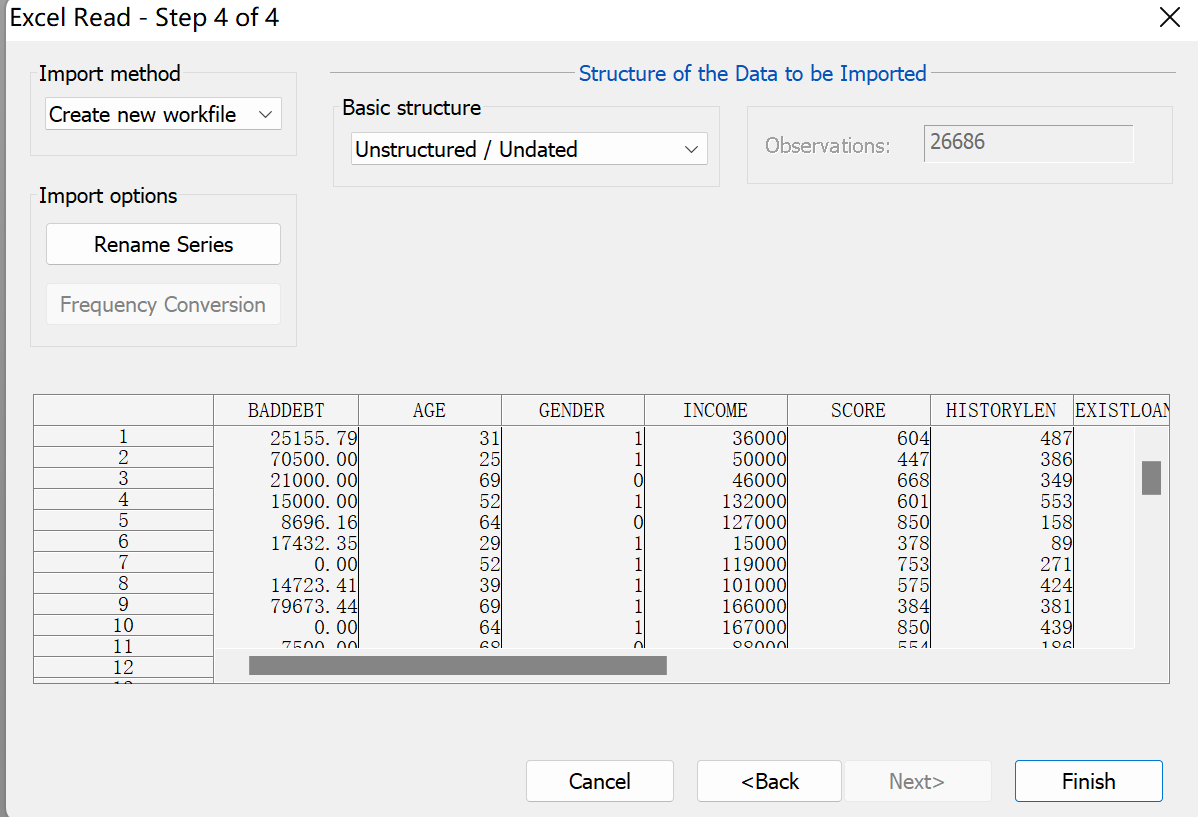
\includegraphics[width=0.7\linewidth]{figures//2DATABASE//db2/导入数据模型2.png}
    \caption{导入数据步骤}
    \label{导入数据模型2}
\end{figure}


本数据集的全部变量的解释如表\ref{数据集II变量组成描述}所示:
\begin{table}[!htbp]
    \setlength{\belowcaptionskip}{0.2cm}
    \centering
    \caption{数据集II变量组成描述}
    \begin{threeparttable}
    \begin{tabular}{c  | p{5cm} |p{7cm}}
    \hline
        \textbf{变量名} & \textbf{解释} & \textbf{取值} \\
        \hline
        \texttt{BadDebt}  & 坏账金额 & 浮点数 \\
        \texttt{Gend}  & 借款人的性别 & 虚拟变量,男性为1,女性则为0 \\
        \texttt{Age}  & 借款人年龄  &整数 \\
        \texttt{Income}  & 借款人的收入 & 整数 \\
        \texttt{Score}  & 信用评分\tnote{*} & 整数 \\
        \texttt{HistoryLen}  & 距首次登记时长(单位:月) & 整数 \\
        \texttt{OldCustomer}  & 是否是本机构老用户 & 虚拟变量,是为1,否则为0 \\
        \texttt{ExistLoan}  & 名下共有贷款数\tnote{**} & 整数 \\
        \texttt{Asset}  & 个人拥有的资产 & 整数 \\
         \texttt{Amount}  & 申请金额 & 整数 \\
         \texttt{T}  & 偿还时间(单位:月) & 整数 \\
         \texttt{Job}  & 是否拥有工作 & 虚拟变量,是为1,否则为0 \\
        \hline
    \end{tabular}
    \label{数据集II变量组成描述}
     \begin{tablenotes}
        \footnotesize
        \item[*] 根据申请人的信用记录量化得出的信用分数,\textbf{分数量化标准与贷款人情况不相干,因此不考虑其与如年龄等个人因素存在多重共线性,但可能和名下贷款数等财务情况相关,需检验},范围在300至850,由信贷机构给出。
         \item[**] 名下共有贷款数包括在其他机构的还款中的贷款数量,不包括已经还清的贷款。

      \end{tablenotes}
    \end{threeparttable}
\end{table}

如图\ref{模型2导入数据2结果}导入结果所示,数据集共含有26686个有效数据。图\ref{模型II的数据分布}显示了各个字段的分布情况。从数据分布来看,年龄、信用评分和名下贷款字段的分布相对均衡,这说明该机构的信用评分体系具有一定的鉴别能力,能够通过不同的借款人信息,较好地区分出信用优良者和潜在风险承担者。另一方面,还款期数和借款金额的分布相对集中,且主要集中在较大金额和较长期限的贷款上。这表明在贷款金额较高和借款周期较长的情况下,违约风险可能更高。这是因为,对于借款人来说,大金额和长期限的贷款意味着更高的还款压力,可能导致还款困难,从而增加违约风险。

\begin{figure}[H]
    \centering
    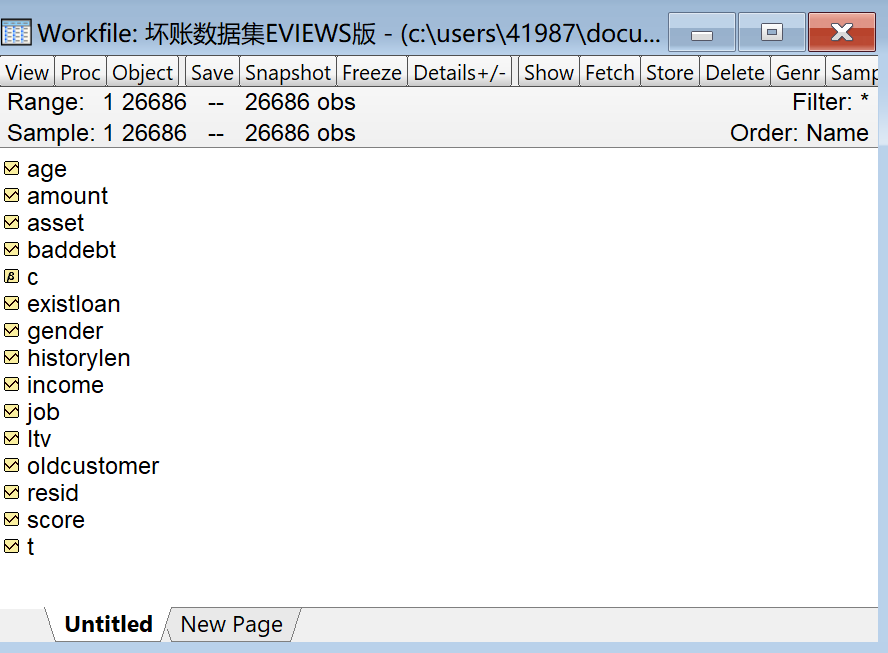
\includegraphics[width=0.7\linewidth]{figures//2DATABASE//db2/导入数据2结果.png}
    \caption{导入数据结果}
    \label{模型2导入数据2结果}
\end{figure}

\begin{figure}[H]
    \centering
    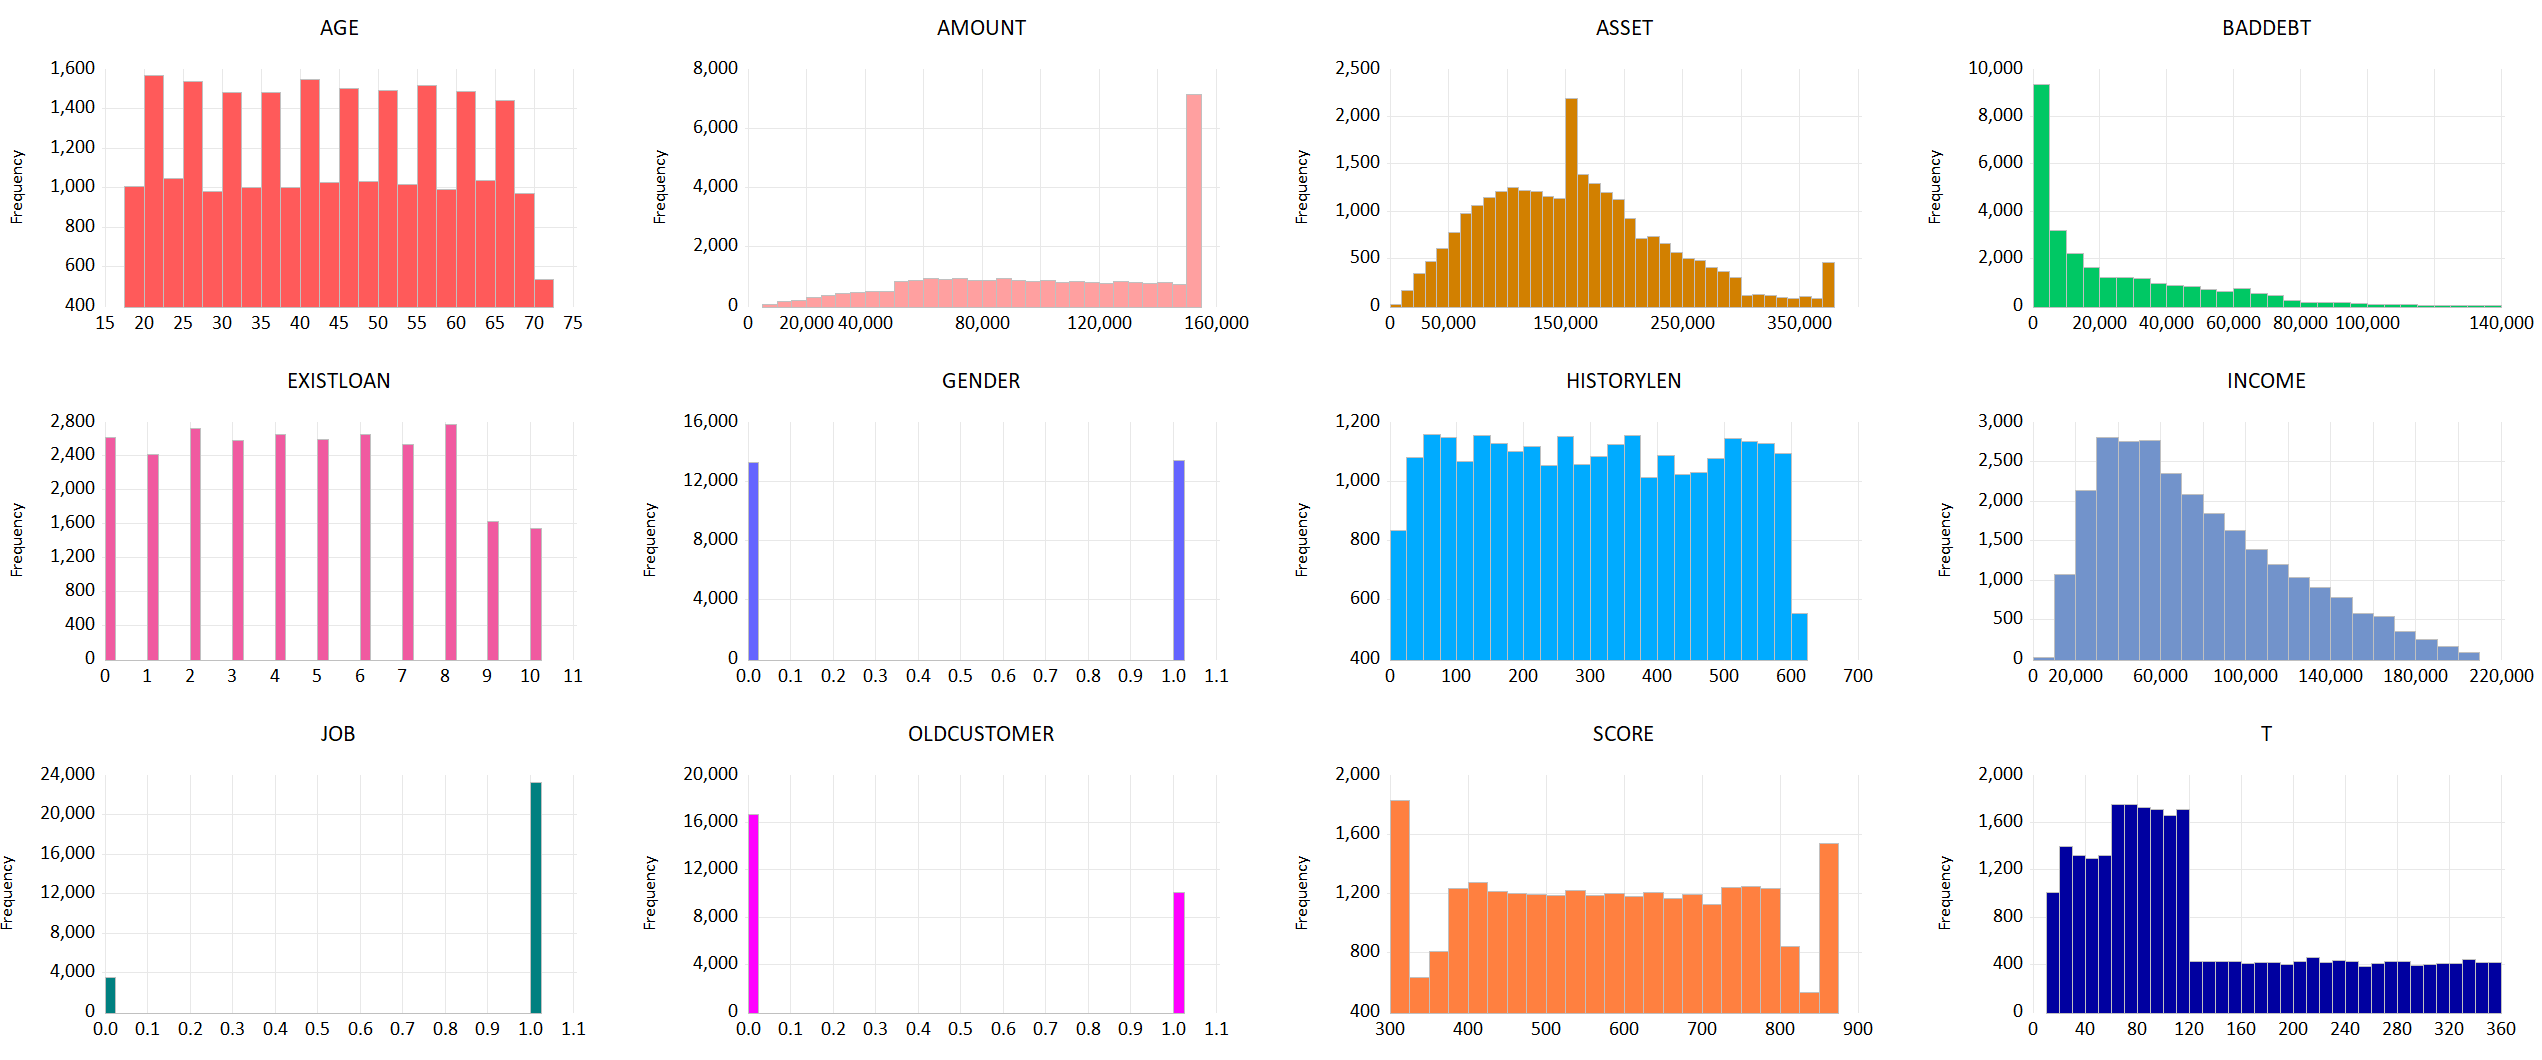
\includegraphics[width=1.1\linewidth]{figures//2DATABASE//db2/模型II的数据分布.png}
    \caption{数据集II:字段数据分布}
    \label{模型II的数据分布}
\end{figure}

在下页表\ref{整数数据样本描述特征模型II}中展示了数据集II中整数数据样本特征。例如,我们可以看到,数据集中平均年龄为43岁,与数据集I基本一致;信用分均值为581左右,位于分布中心;资产情况分布广泛,标准差达到 76390.42,数值较大。各个数据的均值、方差、标准差等均在正常范围以内,认为导入的数据正确无误。

\begin{sidewaystable}[htp]
    \setlength{\belowcaptionskip}{0.2cm}
    \centering
    \caption{数据集II:整数数据样本特征}
    \begin{tabular}{|c|c|c|c|c|c|c|c|c|}
    \hline
        \textbf{} & \textbf{AGE} & \textbf{AMOUNT} & \textbf{ASSET} & \textbf{EXISTLOAN} & \textbf{HISTORYLEN} & \textbf{INCOME} & \textbf{SCORE} & \textbf{T} \\ \hline
        \textbf{Mean} & 43.88361 & 105421.1 & 157018.3 & 4.680469 & 307.4901 & 76062.32 & 581.5645 & 132.8584 \\ \hline
        \textbf{Median} & 44.00000 & 110556.5 & 155200.4 & 5.000000 & 306.0000 & 67000.00 & 582.0000 & 100.0000 \\ \hline
        \textbf{Maximum} & 70.00000 & 150000.0 & 375000.0 & 10.00000 & 611.0000 & 209000.0 & 850.0000 & 359.0000 \\ \hline
        \textbf{Minimum} & 18.00000 & 5985.000 & 6878.159 & 0.000000 & 6.000000 & 9000.000 & 300.0000 & 12.00000 \\ \hline
        \textbf{Std. Dev.} & 15.30358 & 40447.73 & 76390.42 & 3.004889 & 175.7420 & 42881.25 & 164.3482 & 95.96814 \\ \hline
        \textbf{Skewness} & 0.004908 & -0.422880 & 0.584653 & 0.064732 & 0.017156 & 0.723864 & -0.025944 & 0.849593 \\ \hline
        \textbf{Kurtosis} & 1.801662 & 1.926964 & 3.150689 & 1.873832 & 1.790392 & 2.788630 & 1.855095 & 2.521296 \\ \hline
        \textbf{} & ~ & ~ & ~ & ~ & ~ & ~ & ~ & ~ \\ \hline
        \textbf{Jarque-Bera} & 1596.834 & 2075.633 & 1545.549 & 1428.831 & 1628.212 & 2380.159 & 1460.503 & 3465.169 \\ \hline
        \textbf{Probability} & 0.000000 & 0.000000 & 0.000000 & 0.000000 & 0.000000 & 0.000000 & 0.000000 & 0.000000 \\ \hline
        \textbf{} & ~ & ~ & ~ & ~ & ~ & ~ & ~ & ~ \\ \hline
        \textbf{Sum} & 1171078. & 2.81E+09 & 4.19E+09 & 124903.0 & 8205681. & 2.03E+09 & 15519631 & 3545459. \\ \hline
        \textbf{Sum Sq. Dev.} & 6249616. & 4.37E+13 & 1.56E+14 & 240948.4 & 8.24E+08 & 4.91E+13 & 7.21E+08 & 2.46E+08 \\ \hline
        \textbf{} & ~ & ~ & ~ & ~ & ~ & ~ & ~ & ~ \\ \hline
        \textbf{Observations} & 26686 & 26686 & 26686 & 26686 & 26686 & 26686 & 26686 & 26686 \\ \hline
    \end{tabular}
    \label{整数数据样本描述特征模型II}
\end{sidewaystable}

\begin{sidewaystable}[htp]
    \setlength{\belowcaptionskip}{0.2cm}
    \centering
    \caption{数据集II:整数数据样本相关系数表}
    \begin{threeparttable}
    \begin{tabular}{|c|c|c|c|c|c|c|c|c|}
    \hline
        \textbf{} & \textbf{AGE} & \textbf{AMOUNT} & \textbf{ASSET} & \textbf{EXISTLOAN} & \textbf{HISTORYLEN} & \textbf{INCOME} & \textbf{SCORE} & \textbf{T} \\ \hline
        \textbf{AGE} & 1.000000 & 0.271171 & 0.238275 & 0.137138 & 0.003965 & 0.625455 & 0.137470 & 0.073296 \\ \hline
        \textbf{AMOUNT} & 0.271171 & 1.000000 & \textbf{\underline{0.801459}} & 0.086326 & 0.006340 & 0.390543 & 0.086059 & 0.049266 \\ \hline
        \textbf{ASSET} & 0.238275 & \textbf{\underline{0.801459}} & 1.000000 & 0.297150 & 0.007703 & 0.351110 & 0.296299 & 0.192803 \\ \hline
        \textbf{EXISTLOAN} & 0.137138 & 0.086326 & 0.297150 & 1.000000 & 0.001809 & 0.223387 & \textbf{\underline{0.994621}} & 0.645556 \\ \hline
        \textbf{HISTORYLEN} & 0.003965 & 0.006340 & 0.007703 & 0.001809 & 1.000000 & 0.008078 & 0.002491 & -0.007034 \\ \hline
        \textbf{INCOME} & 0.625455 & 0.390543 & 0.351110 & 0.223387 & 0.008078 & 1.000000 & 0.223245 & 0.109349 \\ \hline
        \textbf{SCORE} & 0.137470 & 0.086059 & 0.296299 & \textbf{\underline{0.994621}} & 0.002491 & 0.223245 & 1.000000 & 0.649629 \\ \hline
        \textbf{T} & 0.073296 & 0.049266 & 0.192803 & 0.645556 & -0.007034 & 0.109349 & 0.649629 & 1.000000 \\ \hline
    \end{tabular}
    \label{整数数据样本相关系数表(数据集2)}
    \begin{tablenotes}
        \footnotesize
        \item[*] 受限与版面原因,无法展示各虚拟变量与其他变量的相关系数,但是他们都是小于0.8的  %此处加入注释*信息

      \end{tablenotes}
    \end{threeparttable}
\end{sidewaystable}

在上页表\ref{整数数据样本相关系数表(数据集2)}展示了数据集II中整数数据之间的的相关系数,可以看到,存在两个变量的相关系数较高。

首先,在分析数据时,我们发现\texttt{ExisitLoan}和\texttt{Score}两个变量之间存在高度相关性。具体来说,这两个变量之间的相关系数高达 0.99。在统计学中,相关系数的取值范围在 -1 到 1 之间,值越接近 1,表示两个变量之间的正相关性越强。在这种情况下,我们可以认为评分者在对借款人进行评分时,很大程度上参考了借款人名下的贷款数量。因此,在后续变量选取时,只能选择其中之一。

其次,对于\texttt{Asset}和\texttt{Amount}两个变量,其相关系数达 0.801459,也表明其存在一定的相关性。这是因为借款人的资产状况也可能影响其借款需求。资产总额较大的借款人可能更有动力借款来进行投资、扩大生产等,从而使得资产总额与贷款金额呈正相关。而资产总额较小的借款人,借款需求可能相对较低,贷款金额也较小。

因此,在后续变量选取时,也只能选择其中之一,或者根据相关文献所述,通过\texttt{ltv}值(债务资产比)进行变量代换。该变量代表个人债务与资产之间的比值,与模型I的\texttt{ita}相同,均旨在衡量个体所承受的还款压力。较低的债务资产比意味着借款人承担的还款压力较小,坏账风险较低;相反,较高的债务资产比则表示借款人承受较大的还款压力,坏账风险较高。

由于版面原因,我们没有办法展示虚拟变量之间的相关系数和数据描述,但是经过我们的实操,发现各个虚拟变量与其他变量的相关系数均小于0.8。



\newpage
\section{模型建立与诊断}
本节主要讲述了还款能力和坏账估计两个模型的具体建立流程。对于每个模型,我们会从变量选取触发,进行初步建立,随后诊断模型中存在的各类可能问题(包括多重共线性、异方差、遗漏变量等),进行调整修正,得出最后的回归结果。

\subsection{模型I:还款能力模型}
\subsubsection{变量预期}

首先,我们对各个变量的预期符号提出假设预期。预期结果与解释如表\ref{模型I各变量符号预期}所示。注意,被解释变量TARGET取值为1代表存在还款困难的情况。
\begin{longtable}{|c|p{2cm}<{\centering}|p{9cm}|}
\caption{模型I各变量符号预期} \label{模型I各变量符号预期} \\
\hline
 \textbf{变量名} & \textbf{预期符号} & \textbf{解释} \\
\hline 
\endfirsthead
\multicolumn{3}{l}%
{{\bfseries  续表:}} \\

\hline
 \textbf{变量名} & \textbf{预期符号} & \textbf{解释} \\
\hline 
\endhead
\hline \multicolumn{3}{|r|}{{接下一页}} \\ \hline
\endfoot

\endlastfoot
         \texttt{age}  & $-$ &随着年龄的增长,个人的收入稳定性降低,坏账比例增加。 \\
         \texttt{annamount}  & $-$ & 每年需要还款金额越多,那么还款压力越大,越容易逾期 \\
        \texttt{income}  & + & 收入越高,那么还款压力越小,越不容易逾期 \\
        \texttt{ita}  & $-$ & 收入债务比,值越高,债务越少,收入越高,还款压力小,不容易逾期 \\
        \texttt{gend}  & ? & 无法预期 \\
        \texttt{family}  & + & 家庭人口数量越多,照顾家庭开支可能更大,还款压力大,更可能发生逾期 \\
        \texttt{children}  & + & 子女数量越多,照顾子女的开支可能更大,还款压力大,更可能发生逾期 \\
        \texttt{graduate} & ? & 无法预期,一方面受过高等教育的对自己的财务可能有严格规划,其法律意识、信用意识等更加清晰;另一方面,受到高等教育可能在求学过程中承受较大的经济压力,为完成学业而借款,并且高学历也不一定能获得高收入(如文科类专业)。\\
        \texttt{marry}  & ? & 无法预期,一方面婚后需要照顾家庭,还款压力高,容易逾期;另一方面,结婚后的人群相比未结婚的人群对消费更具有谨慎性和理性,不会毫无计划的乱花钱。 \\
        \texttt{car}  &$-$ & 拥有汽车证明其财务水平较好。\\
        \texttt{house}  & $-$ & 拥有公寓证明其财务水平较好。\\
        \texttt{population}  & $-$ & 人口越多,意味着整体经济发展水平较高,居民收入水平相对较高。较高的收入水平有利于居民按时还款,降低逾期风险。\\
        \texttt{rich}  & $-$ & 整体经济发展水平较高,居民收入水平相对较高。较高的收入水平有利于居民按时还款,降低逾期风险。\\
        \texttt{poverty}  & + & 整体经济发展水平低,居民收入水平相对不高。不利于居民按时还款。\\
        \hline
% ... 更多的行
\end{longtable}

鉴于本研究的自变量为虚拟变量(最终是否成功还款),为了更为精确地预测和解析这一结果,我们将采用 Logit 回归模型进行进一步的实证分析。

\subsubsection{初步回归}
首先,为了充分利用数据尽量纳入全部变量作为解释变量。对于具有多重线性的变量,我们选择其中之一纳入(如family和chilren,ita和annamount和income),在Eviews中输入指令\texttt{LS TARGET C AGE ANNAMOUNT CAR CHILDREN GEND GRADUATE HOUSE INCOME MARRY POPULATION RICH POVERTY}进行第一次回归。

由于本模型为含有虚拟应变量的模型,因此还需将模型调整为Logit模型,调整步骤如图\ref{logit模型步骤模型1}所示:

\begin{figure}[H]
    \centering
    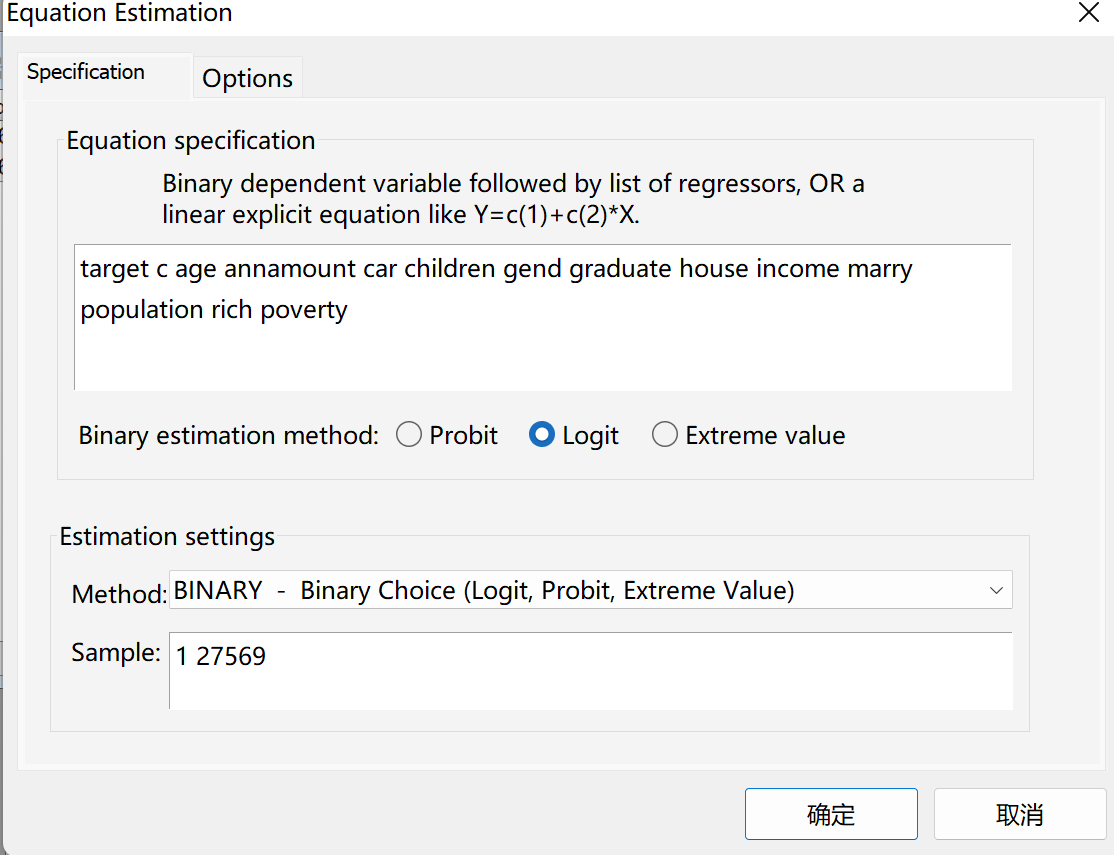
\includegraphics[width =.7\textwidth]{figures/3回归/回归1/logit模型步骤.png}
    \caption{logit模型步骤}
    \label{logit模型步骤模型1}
\end{figure}

回归的结果如下一页图\ref{第一次logit模型}所示。

回归结果为:
\begin{equation}
\begin{split}
 \widehat{L:Pr(TARGET_i=1)}=&-1.25 - 0.03\times AGE + 4.70\times 10^{-6}\times ANNAMOUNT \\ & - 0.29\times CAR + 0.06\times CHILDREN \\ & + 0.42\times GEND - 0.63\times GRADUATE \\ & + 0.04\times HOUSE - 5.41\times10^{-7}\times INCOME \\ & - 0.19\times MARRY + 1.23\times POPULATION \\ & - 0.63\times RICH + 0.39\times POVERTY
\end{split}
\end{equation}


\begin{figure}[H]
    \centering
    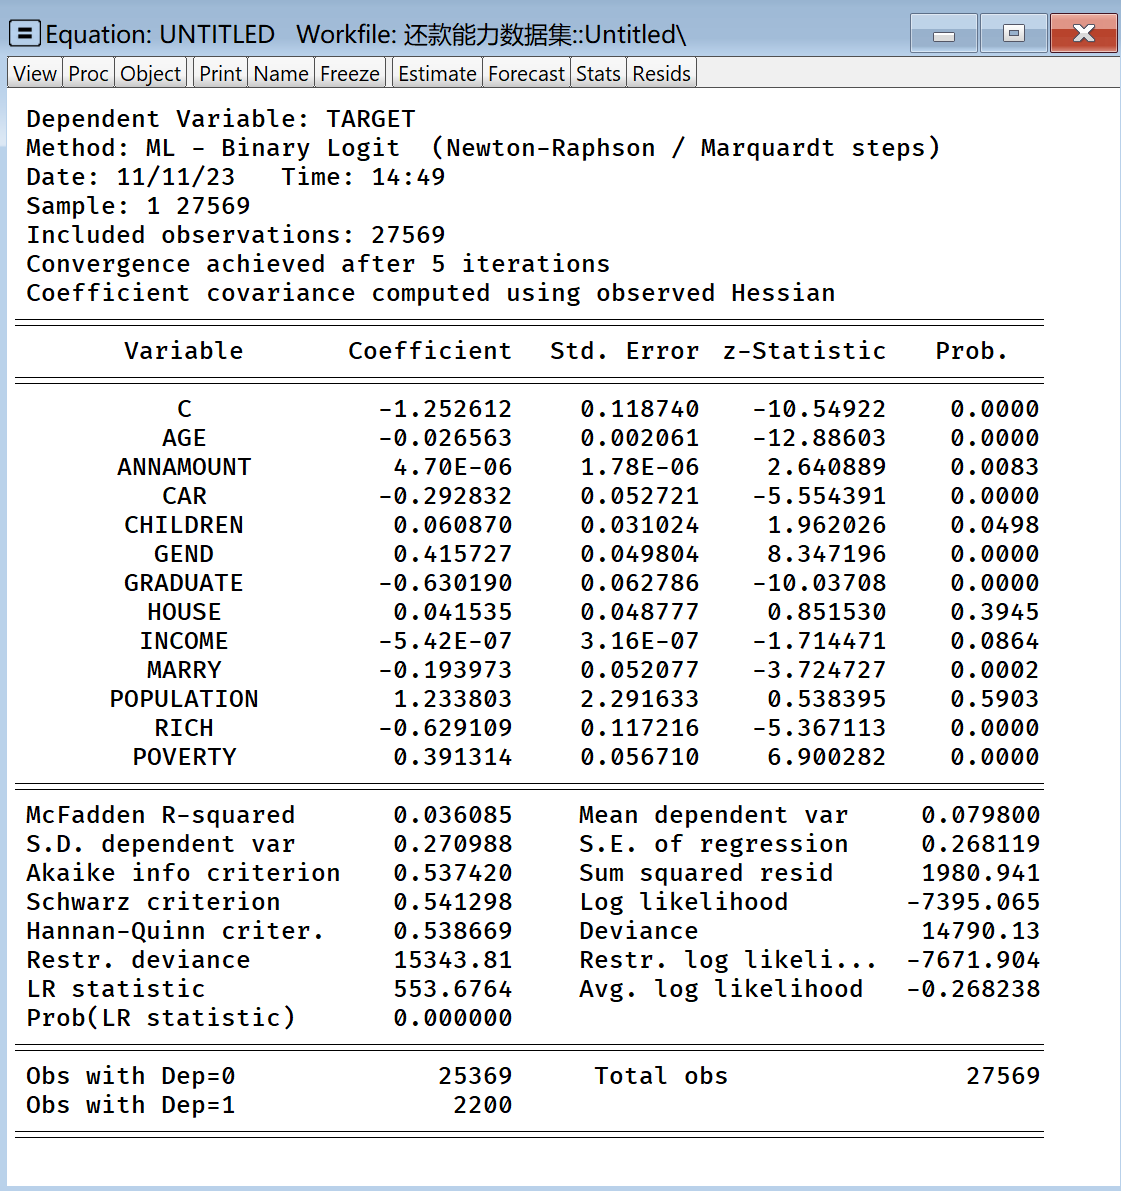
\includegraphics[width=1\linewidth]{figures//3回归//回归1/第一次logit模型.png}
    \caption{模型I初步回归结果}
    \label{第一次logit模型}
\end{figure}

聚焦单独每个变量来看————

首先关注变量 \texttt{house}和\texttt{population}。从预期符号来看,这两个变量的预期符号与实际结果不一致。同时,从显著性水平来看,这两个变量的 z 统计量较低,是所有变量中唯一两个不具备显著性的变量。因此,我们有理由怀疑这两个变量与目标变量之间的关联性不强,可以考虑将它们视为不相干变量。在下一部分将做具体的检验。

接下来,观察变量 \texttt{annamount}和\texttt{income}。虽然这两个变量在模型中具有显著性,但它们的系数较小,对目标变量的影响微乎其微。根据文献资料,更合理的方程设定应该是以收入债务比 \texttt{ita} 代替 \texttt{annamount}和\texttt{income}。


从模型整体来看来看————

模型整体拟合优度McFadden R-squared(即$\overline{R^2_{MCF}}$)为0.036085,拟合程度一般,表明模型中选取的变量对模型有一定的拟合作用,这个模型可以解释目标变量变异的 3.6\%;模型整体显著性水平LR statistic为553.6764,数值远高于临界值,因此,认为模型整体具备显著性。说明模型整体拟合效果较好。





\subsubsection{问题诊断}
通过刚刚的分析,我们认为\texttt{house和population} 这两个变量与目标变量的关联性较弱,可以考虑在构建模型时将其排除。而 \texttt{annamount}和\texttt{income}的系数较小,用收入债务比 \texttt{ita}代替它们能够更好地反映变量间的关联。下面具体来探究这两个优化的正确性与科学性。

\subparagraph {A. 不相干变量:\texttt{house}和\texttt{population}} 
\

下面,依次检验\texttt{house}和\texttt{population}是否为冗余变量。
在 Eviews 软件中,我们按照顺序选择 Coefficient Diagnostics -> Redundant Variables Test

\begin{figure}[H]
    \centering
    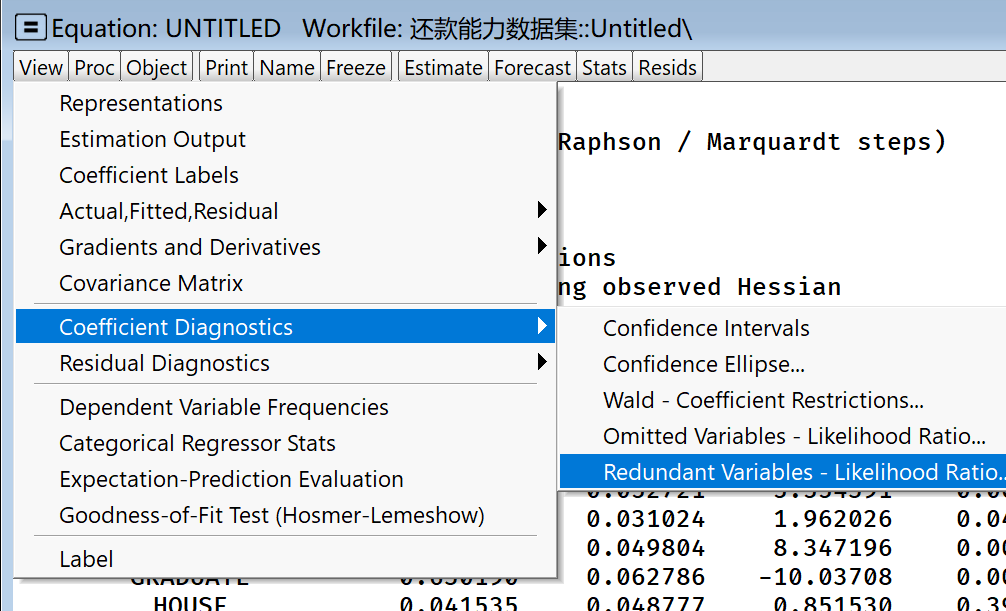
\includegraphics[width=0.5\linewidth]{figures//3回归//回归1/冗余检查步骤.png}
    \caption{冗余检查步骤}
    \label{冗余检查步骤模型1}
\end{figure}
建立假设
\begin{equation}
    \begin{split}
        H_0:& 变量house和population是冗余变量 \\
        H_A:& H_0不成立 \nonumber
    \end{split}
\end{equation}

在输入框中输入\texttt{house}和\texttt{population},进行检验

检验结果如图\ref{house和population是冗余变量.png}所示:

\begin{figure}[H]
    \centering
    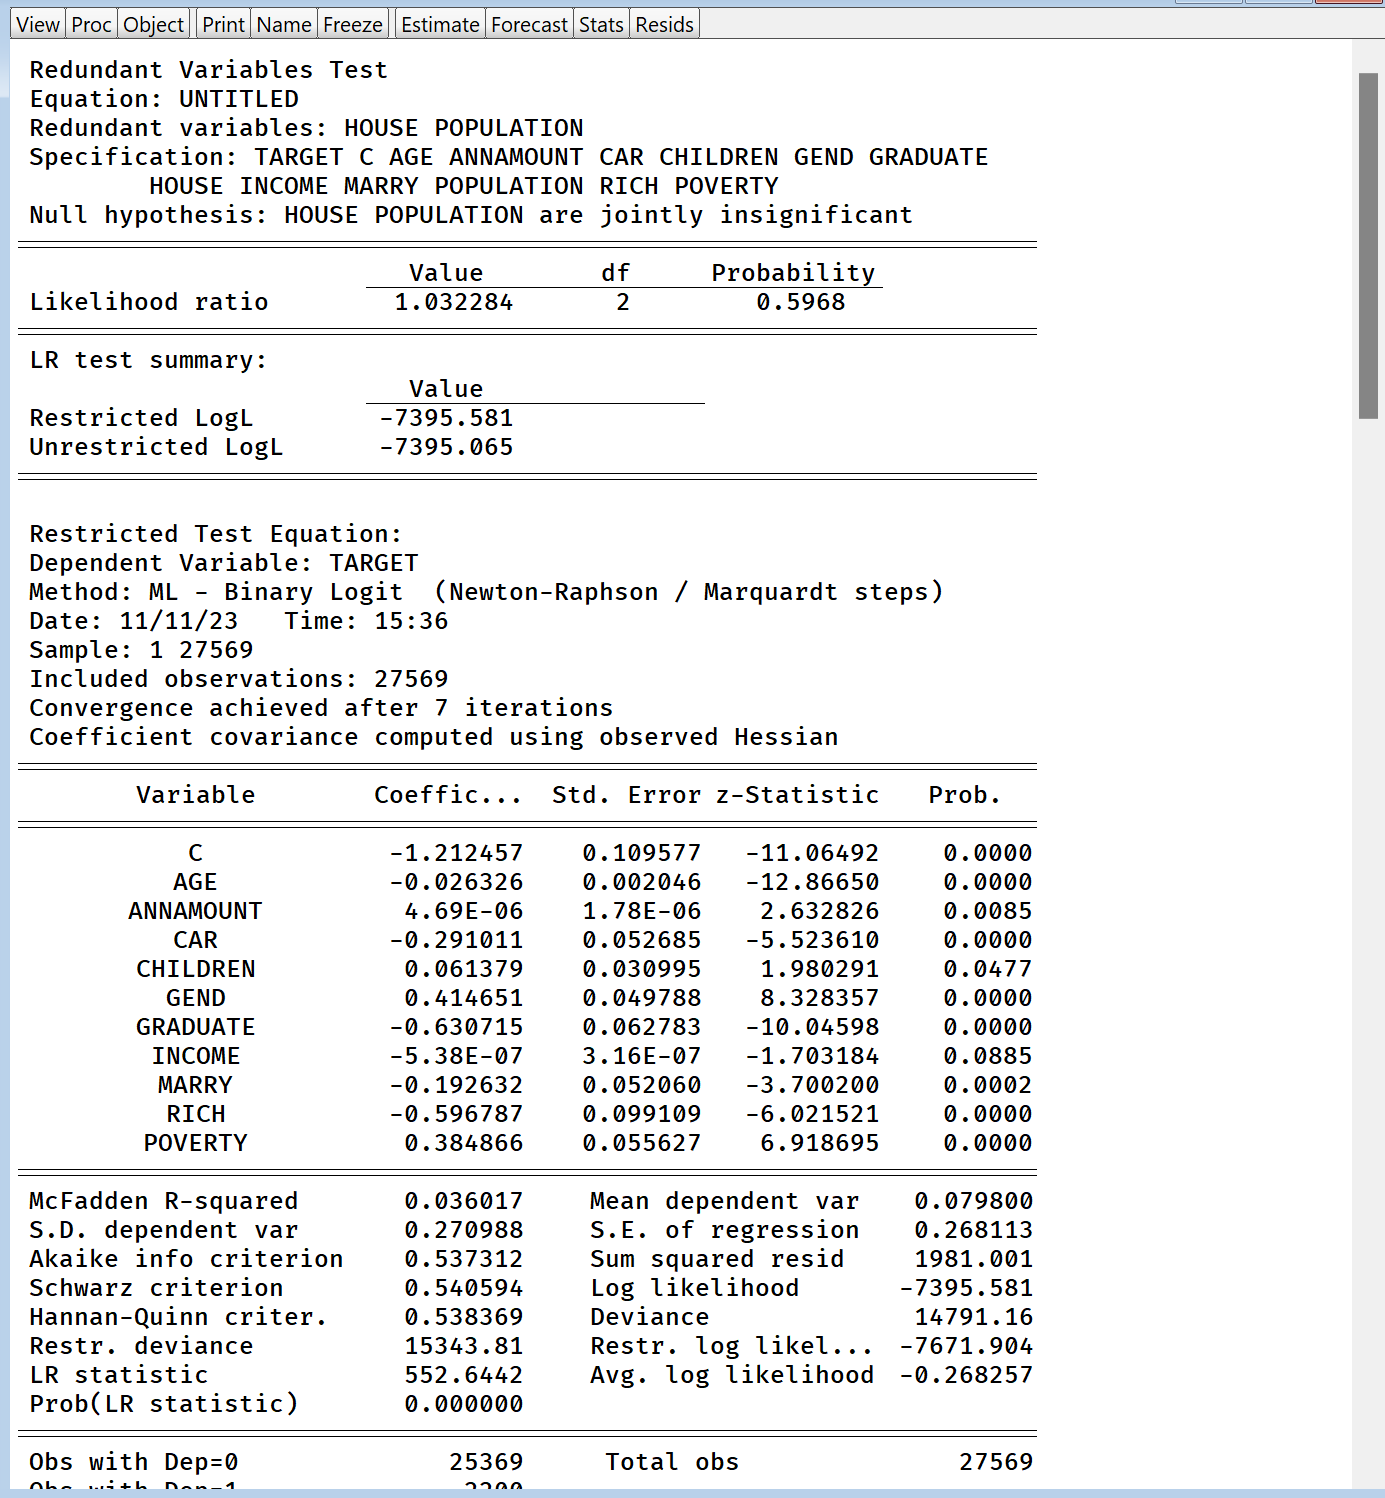
\includegraphics[width=1\linewidth]{figures//3回归//回归1/house和population是冗余变量.png}
    \caption{模型I冗余变量检查结果}
    \label{house和population是冗余变量.png}
\end{figure}

根据检验结果,我们可以发现,似然比低于临界值,p值远高于显著性水平5\%,因此不能拒绝原假设$H_0$,\textbf{所以可以认为\texttt{house}和\texttt{population}是一个不相干变量}。应该将其剔除。

从理论再次分析,首先,\texttt{house}变量原本应作为借款人财务状况的衡量标准,然而在实际操作中,鉴于年轻人在购房方面的特殊处境,这一变量并未充分体现其财务实力。购房对于年轻人来说通常是必需的,而这方面的资金往往来源于父母、亲戚、朋友等资助。这样一来,拥房与否并不能直接反映一个人的财务状况。相反,汽车作为非必需消费品,一般情况下是在购房之后,年轻人在经济允许的情况下自费购买,受他人资助较少。因此,拥有汽车能够更好地体现出一个人的经济实力。

根据\cite{汽车消费、住房抵押贷款违约特性及对策}的研究,这一观点得到了证实。尽管\texttt{house}这个变量看似合理,但实际上却没有解释效力。综上所述,我们在分析借款人财务状况时,应当关注其是否拥有汽车,而不仅仅是房子。

其次,\texttt{population}这一因素用于反映借款人所处城市收入水平并不恰当。因为人口数量与城市财富水平之间并非完全正相关,人口众多并不代表人均收入较高。根据文献\cite{中国省级人口增长率和GDP增长率及其相关关系研究}的研究,对于大部分中等发达地区和一部分欠发达地区,人口数量与 GDP 确实存在正相关关系。然而,在大多数发达地区和部分欠发达地区,人口增长率与 GDP 增长率呈现负相关。因此,人口并非是衡量城市收入水平、物价等经济因素的理想指标。

\subparagraph {B. 变量设定: \texttt{ita}代替\texttt{annamount}和\texttt{income}}
\

我们首先检测\texttt{ita}是否是遗漏变量。
\begin{figure}[H]
    \centering
    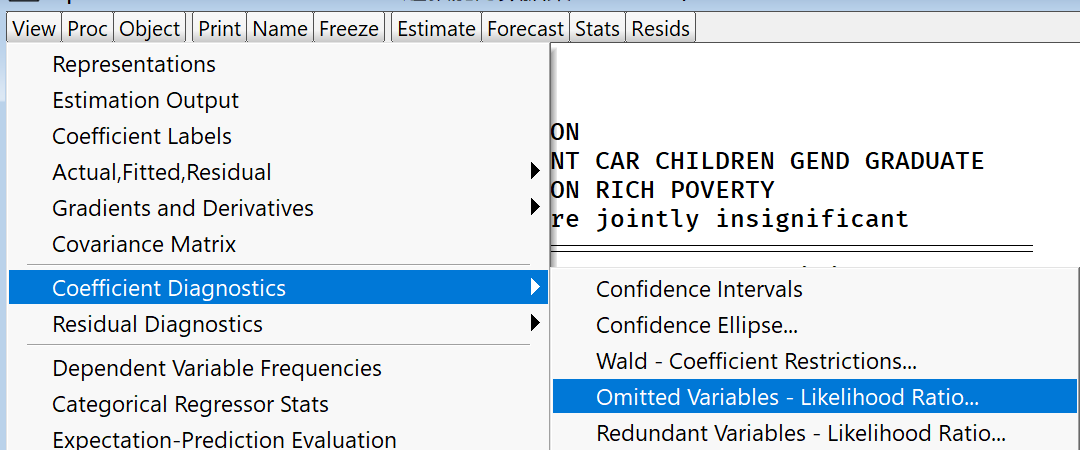
\includegraphics[width=0.5\linewidth]{figures//3回归//回归1/遗漏变量.png}
    \caption{遗漏变量检测步骤}
    \label{遗漏变量检测步骤模型1}
\end{figure}

在 Eviews 软件中,我们按照顺序选择 Coefficient Diagnostics -> Omitted Variables Test 菜单。
建立假设
\begin{equation}
    \begin{split}
        H_0:& 变量ita不是遗漏变量 \\
        H_A:& H_0不成立 \nonumber
    \end{split}
\end{equation}

检验结果如图\ref{遗漏变量检测结果模型1}所示:

\begin{figure}[H]
    \centering
    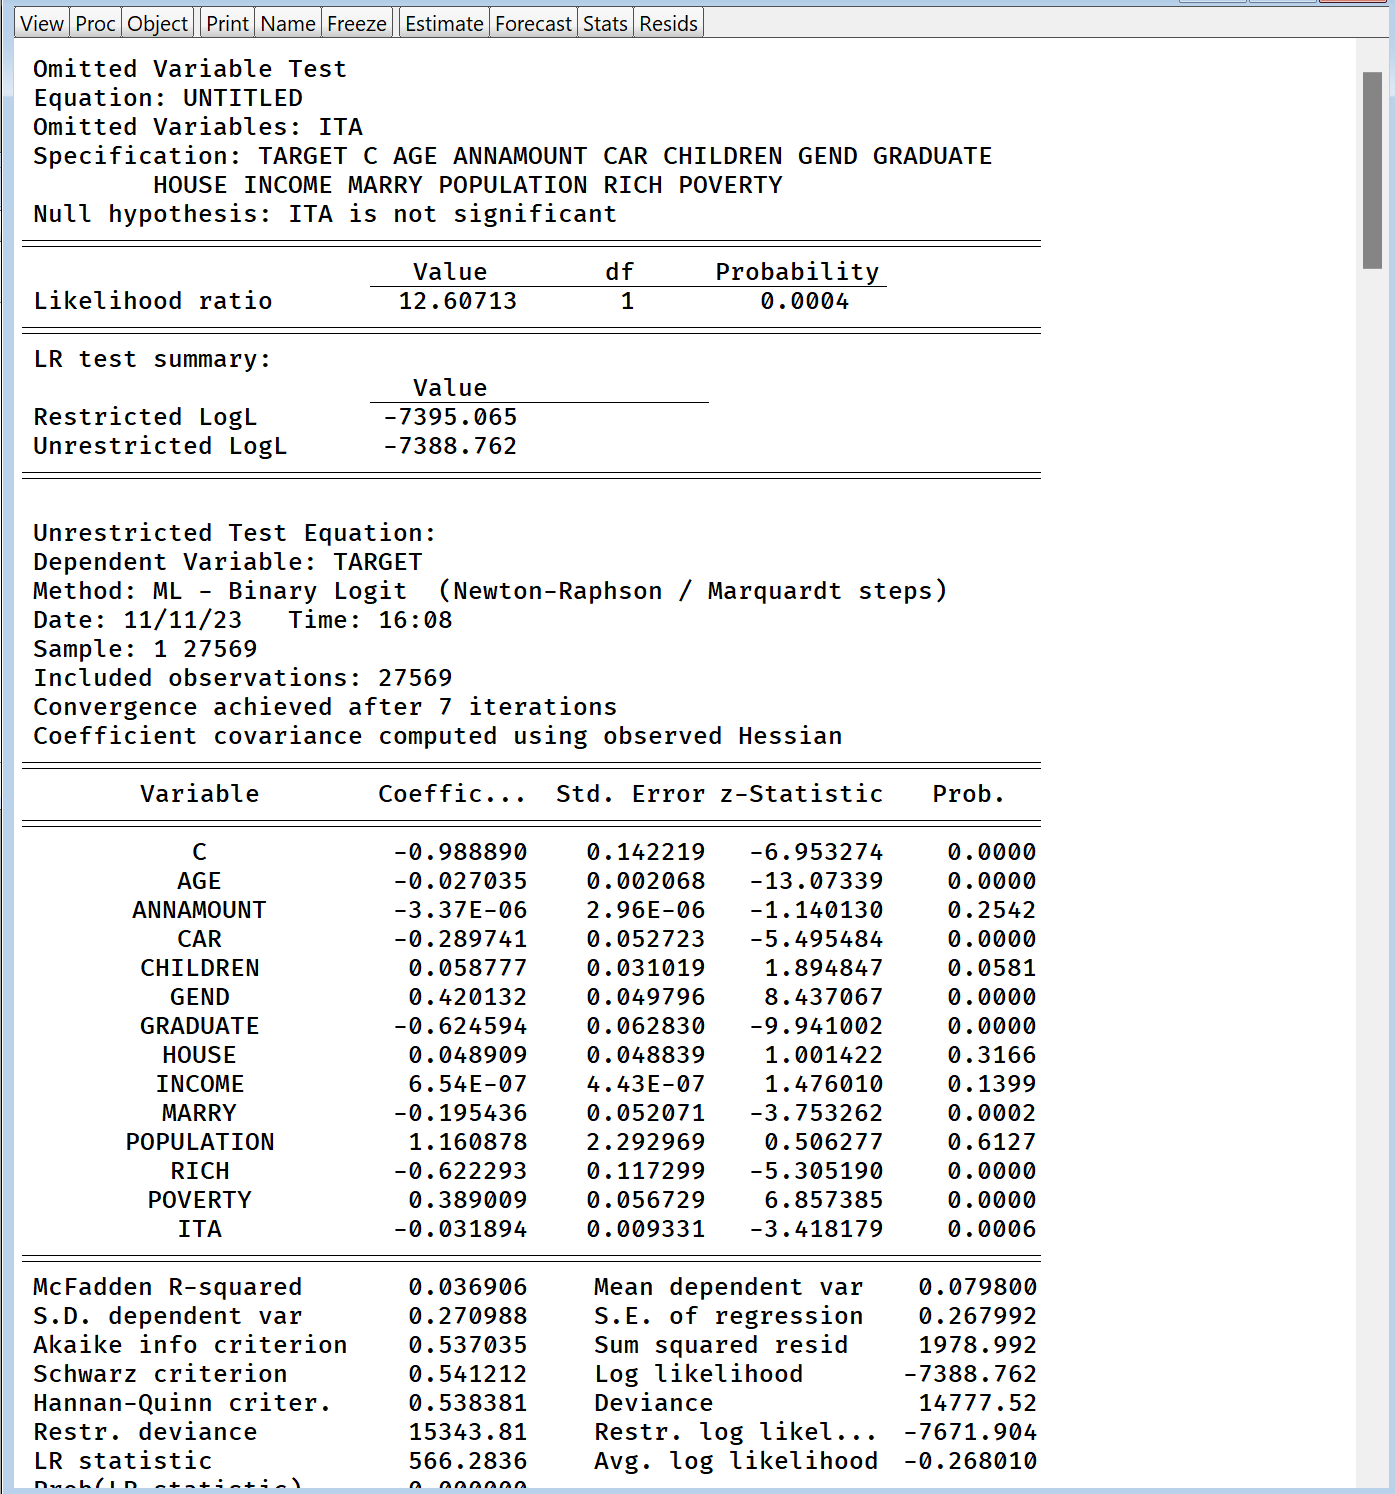
\includegraphics[width=1\linewidth]{figures//3回归//回归1/遗漏变量ita结果.png}
    \caption{遗漏变量检测结果}
    \label{遗漏变量检测结果模型1}
\end{figure}

根据检验结果,我们可以发现,p值<显著性水平5\%,所以\textbf{可以认为\texttt{ita}是一个遗漏变量}。

\texttt{ita}这个变量具有深刻的理论意义,它通过衡量人们的收入与还款金额之间的比例关系,揭示了一种衡量借款人还款压力的有效方法。这一点已经在第一部分的理论中阐述,不再此处赘述。这个变量在一定程度上反映了借款人的经济状况和对债务的承担能力,从而为贷款评估有力的支持。因此,将其纳入模型是必然的选择。

当然,由于\texttt{ita}是由\texttt{income}、\texttt{annamount}计算而来,因此\texttt{ita}和\texttt{income}、\texttt{annamount}存在一定的多重共线性。基于此,\textbf{我们选择用\texttt{ita}代替\texttt{annamount}和\texttt{income}}。


\subsubsection{模型修正}

下面,根据我们的诊断结果,我们对模型I进行进一步的调整和修正,使得其拟合效果更加、经济理论意义更好。

在Eviews中输入指令\texttt{LS TARGET C AGE CAR CHILDREN GEND GRADUATE MARRY RICH POVERTY ITA}进行修正回归。整个修正中,我们删掉了\texttt{house}和\texttt{population}两个冗余变量,同时用\texttt{ita}代替\texttt{annamount}和\texttt{income}。由于本模型为含有虚拟应变量的模型,因此还需将模型调整为Logit模型,回归结果如下一页图\ref{修正后的回归结果模型1}所示。

模型回归结果为————

\begin{equation}
    \begin{split}
        \widehat{L:Pr(TARGET_i=1)}=&-0.70 - 0.01\times AGE - 0.14\times CAR \\ &  + 0.03\times CHILDREN + 0.22\times GEND \\ & - 0.30\times GRADUATE - 0.10\times MARRY - 0.28\times RICH \\ &  + 0.19\times POVERTY - 0.01\times ITA
    \end{split}
\end{equation}

\begin{figure}[H]
    \centering
    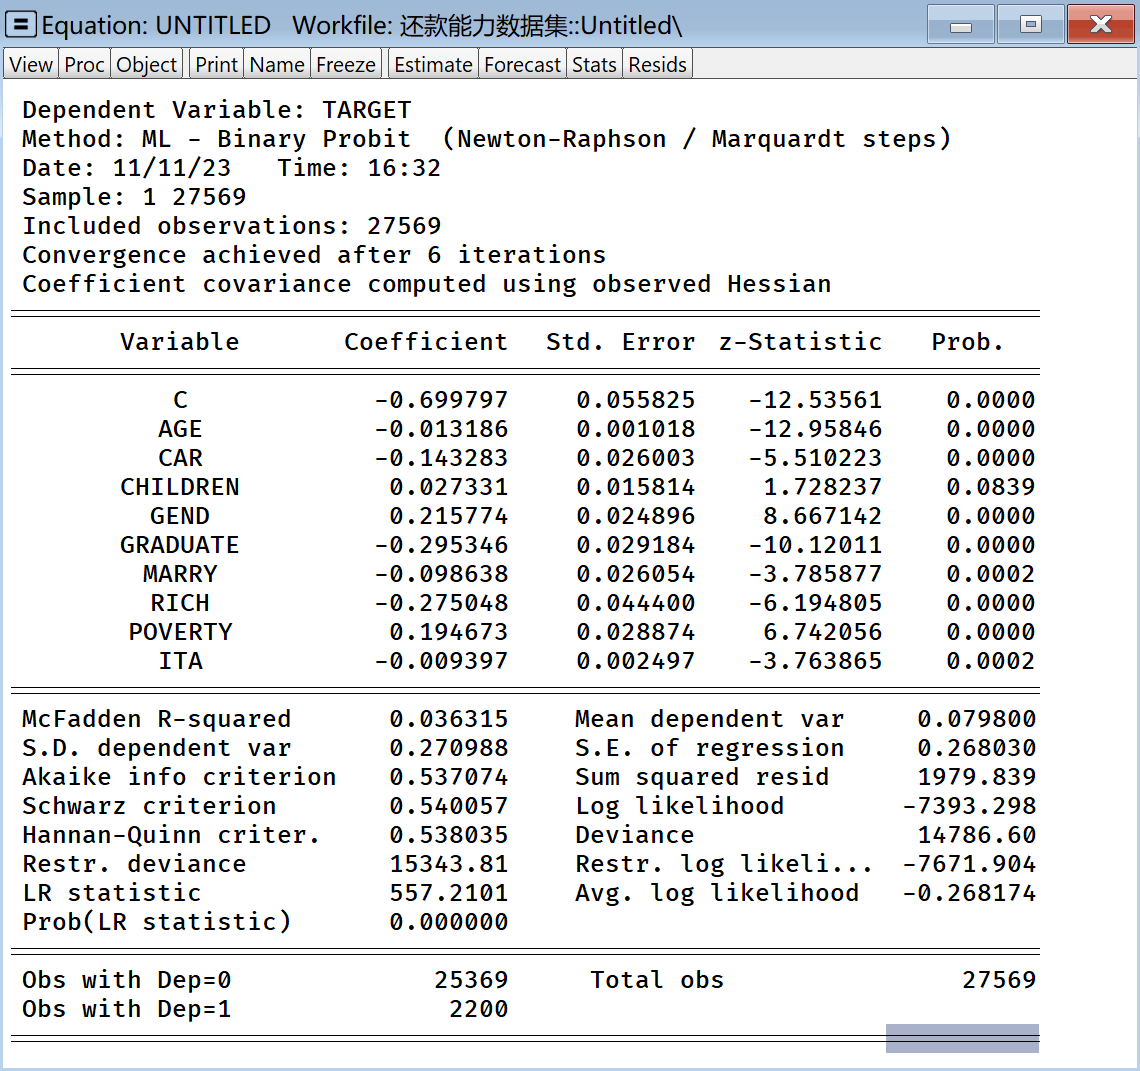
\includegraphics[width=1\linewidth]{figures//3回归//回归1/修正回归.png}
    \caption{修正后的回归结果}
    \label{修正后的回归结果模型1}
\end{figure}

从模型设定的四个角度来看:

\quad \textbf{(a) 理论:}\quad 去除冗余变量\texttt{house}和\texttt{population}、用\texttt{ita}代替\texttt{annamount}和\texttt{income}这两个操作均具有实际的理论意义。\texttt{ita}可以直观的反应借款者的还款压力,从而更好的衡量借款者的还款能力。具备经济理论基础。

\quad \textbf{(b) 显著性: }\quad 在5\%的显著性条件下,所有变量其余的变量均变得完全显著。(因为Eviews是双侧检验,对于\texttt{children}变量,$p/2<5\%$仍然成立)。单个变量的显著性上提升较大;同时,LR值也由原来的553提升到现在的557,整体显著性上也有一定的提升。

\quad \textbf{(c) 拟合优度: }\quad 整体拟合优度由原来的0.036085提升到0.036315,有略微的提升,模型的拟合效果更好了。

\quad \textbf{(d) 偏误: }\quad 对比前后两个模型,各个系数的偏误不大。

综上,修复后的模型解决了我们刚刚检查出的两个问题,并在显著性、拟合优度上有一定程度提升,更具备理论意义。

模型的具体经济意义我们将在第4节详细论述。


\subsection{模型II:坏账金额模型}
\subsubsection{变量预期}

首先,我们对各个变量的预期符号提出假设预期。预期结果与解释如表\ref{模型II各变量符号预期}所示。

\begin{longtable}{|c|p{2cm}<{\centering}|p{9cm}|}
\caption{模型II各变量符号预期} \label{模型II各变量符号预期} \\
\hline
 \textbf{变量名} & \textbf{预期符号} & \textbf{解释} \\
\hline 
\endfirsthead
\multicolumn{3}{l}%
{{\bfseries  续表:}} \\

\hline
 \textbf{变量名} & \textbf{预期符号} & \textbf{解释} \\
\hline 
\endhead
\hline \multicolumn{3}{|r|}{{接下一页}} \\ \hline
\endfoot

\endlastfoot
         \texttt{age}  & $+$ & 随着年龄的增长,个人的收入稳定性降低,坏账金额增加。 \\
         \texttt{annamount}  & $+$ & 每年需要还款金额越多,那么还款压力越大,坏账金额增加。\\
         \texttt{asset}  & $-$ & 资产数量越多,可用于抵押偿还贷款的金额越多,可能的坏账金额越少 \\
         \texttt{ltv}  & $+$ & 较低的债务资产比意味着借款人承担的还款压力较小,坏账风险较低;相反,较高的债务资产比则表示借款人承受较大的还款压力,坏账风险较高 \\
        \texttt{income}  & $-$ & 收入越高,那么还款压力越小,不容易造成欠款,坏账金额低 \\
        \texttt{gender}  & ? & 无法预期 \\
        \texttt{score}  & $-$ & 信用分越低,其偿还贷款的可能性越低,拥有坏账的可能性越高 \\
        \texttt{t}  & ? & 无法预期,一方面,还款周期越长,借款人有更多的时间去周转,每月还款压力小;同时另一方面,时间越长,不确定性越多,风险可能越高。 \\
        \texttt{existloan}  & $+$ & 现有贷款数越多,需要偿还的数量越多,还款压力越大,坏账比例越高 \\
        \texttt{job}  & $-$ & 拥有稳定工作的人比没有稳定工作的人收入更稳定 \\
        \texttt{historylen}  & $+$ & 信用记录长,信用越可靠,那么坏账的风险越小 \\
        \texttt{oldcustomer}  & ? & 无法预期,一方面,老顾客具有贷款经验,且在过去的交易中建立了良好的信用记录;另一方面,信贷机构可能会对他们产生过度信任,导致在贷款审批过程中放松警惕。 \\
        \hline
% ... 更多的行
\end{longtable}

这是一个典型的可以使用最小二乘法的普通模型,下面,我们对模型进行初步的建立。

\subsubsection{初步回归}

在初次建立模型时,因为遗漏变量往往比不相干变量更严重,因此我们尽可能考虑更多的解释变量,以防遗漏变量带来的一些风险。由于受到多重共线性的影响,我们去掉相关系数最为严重的一组中的\texttt{existloan},保留了\texttt{score}。因为相比前者,\texttt{score}更能全面反应借款者的用户个人情况。

在Eviews中,我们输入指令 \texttt{LS baddebt c age asset amount score oldcustomer t gender income job historylen}开始第一次回归常识

回归的结果如图\ref{第一次回归模型}所示。

\begin{figure}[H]
    \centering
    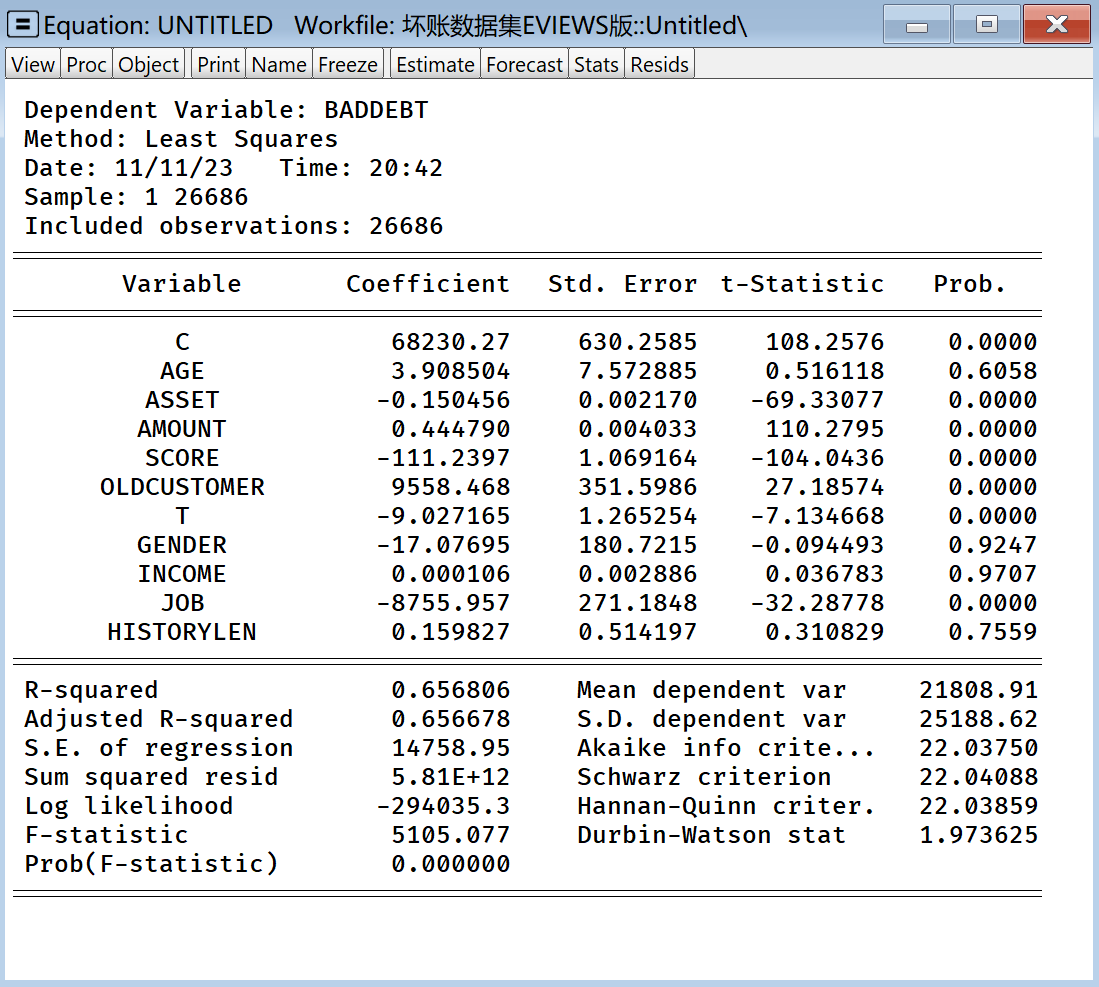
\includegraphics[width=1\linewidth]{figures//3回归//回归2/第一次回归结果.png}
    \caption{模型II初步回归结果}
    \label{第一次回归模型}
\end{figure}

回归结果为:
\begin{equation}
\begin{split}
 BADDEBT &= 68230.27+ 3.91\times AGE - 0.15\times ASSET + 0.44\times AMOUNT \\ & - 111.24\times SCORE + 9558.47\times OLDCUSTOMER \\ & - 9.03\times T - 17.08\times GENDER + 0.000106\times INCOME \\ & - 8755.96\times JOB + 0.16\times HISTORYLEN
\end{split}
\end{equation}

\

下面对回归结果做简要分析。

聚焦单独每个变量来看————

从符号来看,\texttt{income}变量出现了和预期相背离的情况,这可能意味着我们在构建模型时存在一些问题。从显著性水平来看,\texttt{gender}、\texttt{income}、\texttt{historylen}这三个变量,其t值均小于临界值,无法拒绝原假设,这说明我们在当前的模型中并未观察到显著性水平,这可能表明这些变量在预测结果中的作用并不明显,或者我们的模型尚未足够完善。


从模型整体来看来看————

模型整体拟合优度调整的R平方(即$\overline{R^2}$)为0.656806,拟合程度较好,表明模型中选取的变量对模型有不错的拟合作用,这个模型可以解释目标变量变异的 65.6\%;模型整体显著性水平F值为5105.077,数值远高于临界值,因此,认为模型整体具备显著性。说明模型整体拟合效果较好。

模型的整体显著性水平很高,但出现了3个不显著变量与1个预期符号相反的变量,因此,有必要对模型进行诊断。

\subsubsection{问题诊断}
\subparagraph {A. 序列相关性}
\

我们对数据采用LM检验法。首先建立假设:
\begin{equation}
    \begin{split}
        H_0:& 模型存在序列相关性 \\
        H_A:& H_0不成立 \nonumber
    \end{split}
\end{equation}

在线性回归的结果中,依次点击view->Residual Diagnostcis->Serial Correlation LM Test。进行LM检验。我们设定检验的阶数为2。

最终,得到如下页图\ref{序列相关检验II}的检验结果。

从结果可以看到,$nR^2$的结果为4.701187,p值为0.0953,其统计量小于卡方临界值且p值>5\%,因此不能原假设,因此,可以得出结论———\textbf{认为该模型并不存在序列相关性}。

\begin{figure}[H]
    \centering
    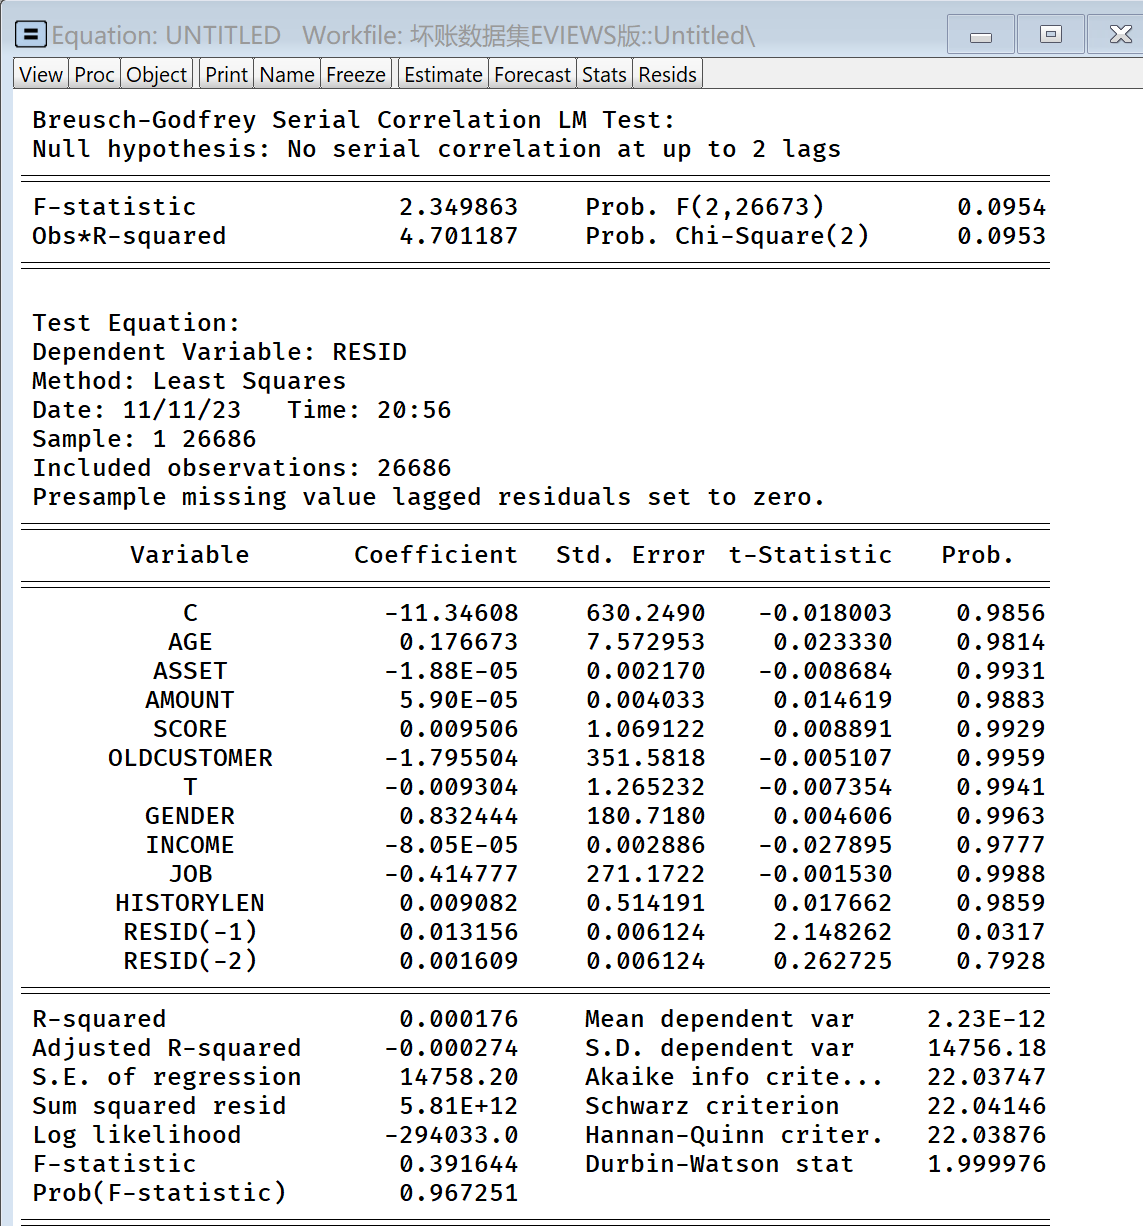
\includegraphics[width=1\linewidth]{figures//3回归//回归2/II序列相关检验.png}
    \caption{序列相关检验}
    \label{序列相关检验II}
\end{figure}


\subparagraph {B. 多重共线性}
\

方程可能存在序列相关性,因为在第二节的相关系数分析中,我们发现\texttt{amount}和\texttt{asset}的相关系数较高。下面对其使用VIF检验。

在 Eviews 软件中,我们选择 View->Coefficient Diagnostics->Variance Inflation Factors 进行方差膨胀因子分析。

\begin{figure}[H]
    \centering
    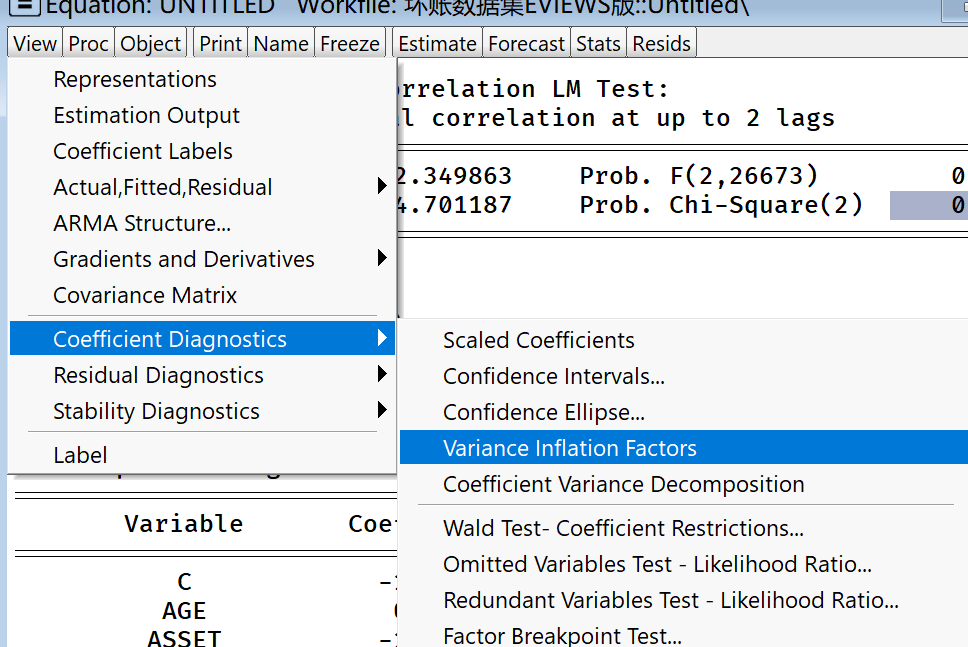
\includegraphics[width=0.5\linewidth]{figures//3回归//回归2/VIF步骤.png}
    \caption{方差膨胀因子查看步骤}
    \label{VIF步骤}
\end{figure}


分析结果如图\ref{方差膨胀因子检验结果}所示。

\begin{figure}[H]
    \centering
    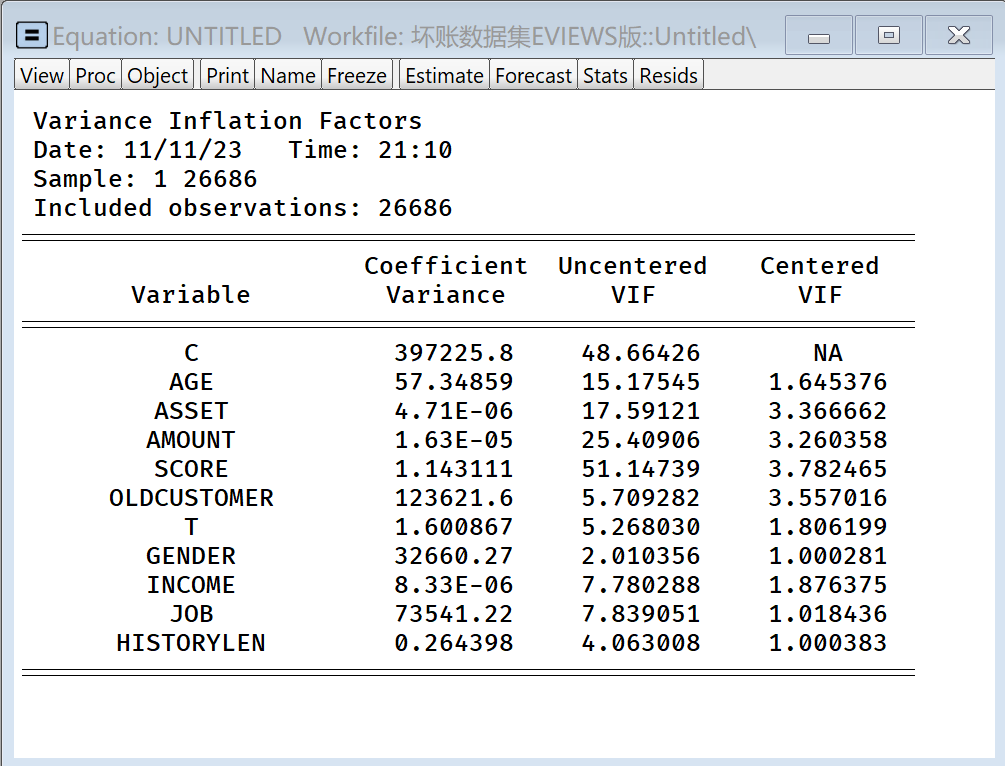
\includegraphics[width=1\linewidth]{figures//3回归//回归2/VIF结果.png}
    \caption{方差膨胀因子检验结果}
    \label{方差膨胀因子检验结果}
\end{figure}

可以看到,所有系数的VIF值均小于5。一般而言,只有VIF(方差膨胀因子)大于五才认为存在明显的多重线性。综上,可以认为\textbf{该模型不存在多重共线性}。

\subparagraph {C. 不相干变量}
\

下面,依次检验\texttt{gender}、\texttt{income}、\texttt{historylen}是否为冗余变量。
在 Eviews 软件中,我们按照顺序选择 Coefficient Diagnostics -> Redundant Variables Test。在输入框中输入\texttt{gender}、\texttt{income}、\texttt{historylen},进行检验

检验结果如图\ref{gender、income、historylen是冗余变量.png}所示:

\begin{figure}[H]
    \centering
    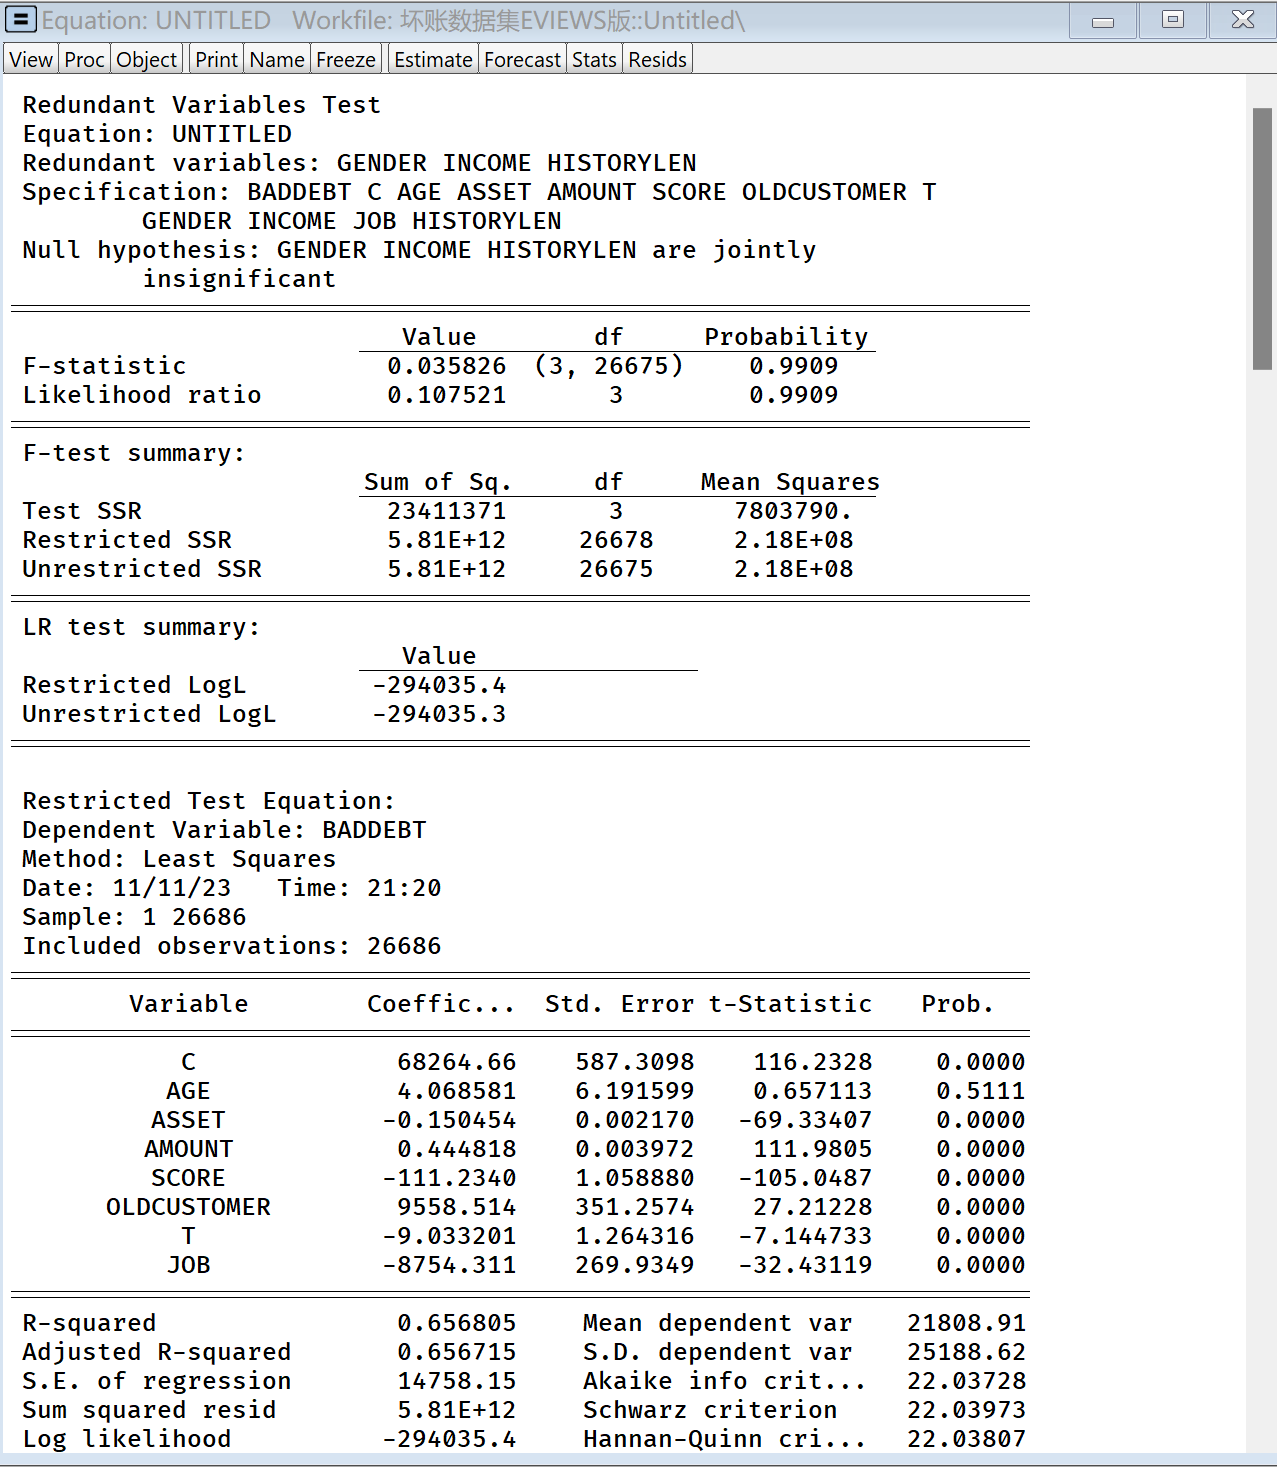
\includegraphics[width=.9\linewidth]{figures//3回归//回归2/模型II冗余.png}
    \caption{模型II冗余变量检查结果}
    \label{gender、income、historylen是冗余变量.png}
\end{figure}

根据检验结果,我们可以发现,F统计量为 0.035826,低于临界值,p值远高于显著性水平5\%,因此不能拒绝原假设$H_0$,\textbf{所以可以认为\texttt{gender}、\texttt{income}、\texttt{historylen}三者均是不相干变量}。应该将其剔除。


从理论角度来看,首先,性别对贷款坏账的影响一直存在广泛的争议,没有明确的结论。性别差异在很大程度上可能是由其他变量所解释的,如收入、职业等。因此,从理论角度来看,性别作为一个独立变量对贷款坏账的预测能力有限,将其剔除可能更为合适。

其次,收入这个变量在理论上也是冗余的。这是因为收入的解释能力可能已经被其他更能反映借款人财务水平的变量所替代,如资产、信用评分等。这些变量能更好地预测借款人的还款能力,从而降低贷款坏账的风险。因此,在模型中包含收入这个变量可能导致信息冗余,影响模型的预测效果。

最后,信用记录(historylen)这个变量也是一个冗余变量。虽然理论上信用历史较长的借款人可能具有较高的还款能力,从而降低贷款坏账的风险,但这个变量仅仅简单地衡量了首次登记距今天的时间长短,并未反映出这期间的信用状况好坏。在其他变量如信用评级、收入等已经能够解释信用历史差异的情况下,这个变量可能显得冗余。

综上所述,从理论角度来看,\texttt{gender}、\texttt{income}、\texttt{historylen}这三个变量都被确认为是冗余变量。需要进行剔除。


\subparagraph {D. 异方差性}
\

该方程可能存在异方差性,因为随着贷款金额的增加,还款金额也就随之越高,如果他的信用较低,那么坏账的总金额也越高,呈现一种规模效应。

我们首先通过图解法简单观察,在Eviews中输入\texttt{SCAT LOG(AMOUNT) RESID}绘制出贷款金额的对数与残差的散点分布图。绘图结果如下一页图\ref{贷款金额的对数与残差的散点分布图}所示。

从图结果可以看到,随着贷款金额的增加,残差也逐步增大。整体呈现着一种上升趋势。综上,可以初步认为该模型存在异方差性

\begin{figure}[H]
    \centering
    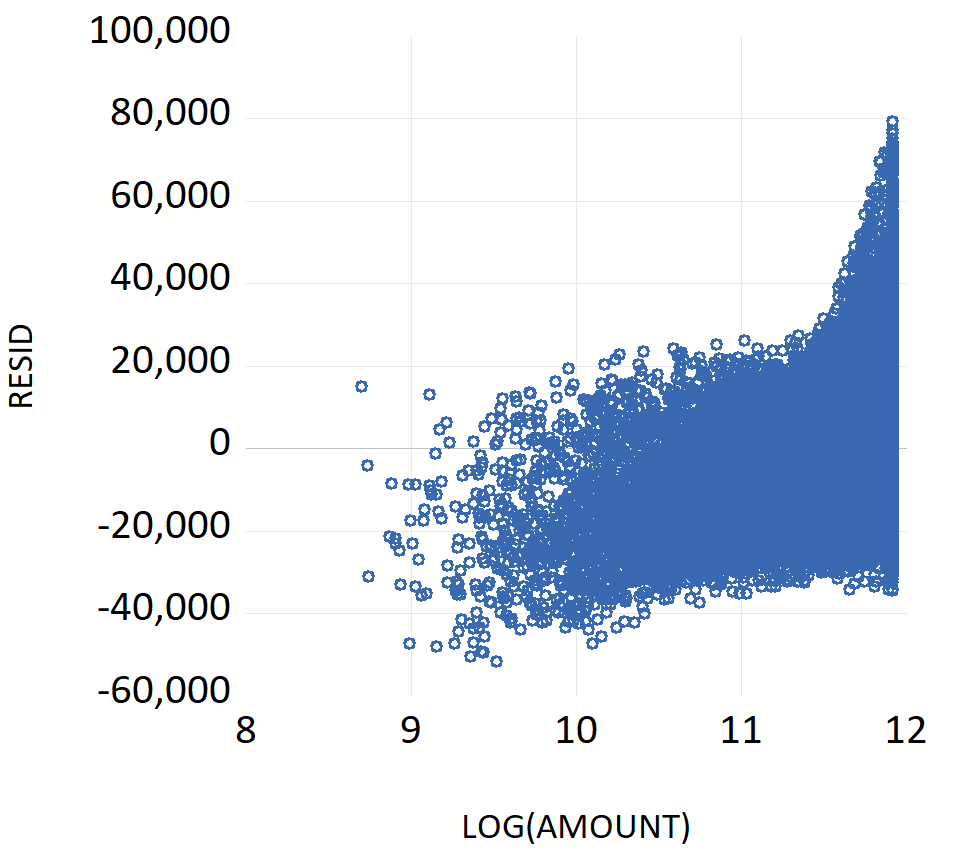
\includegraphics[width=0.75\linewidth]{figures//3回归//回归2/resid散点图.png}
    \caption{贷款金额的对数与残差的散点分布图}
    \label{贷款金额的对数与残差的散点分布图}
\end{figure}

下面,我们通过white检验法进行进一步检验。

在 Eviews 中,我们选择 View 菜单中的 Residual Diagnostics 的 Heteroskedasticity tests 选项,接着选择 White 检验。

\begin{figure}[H]
    \centering
    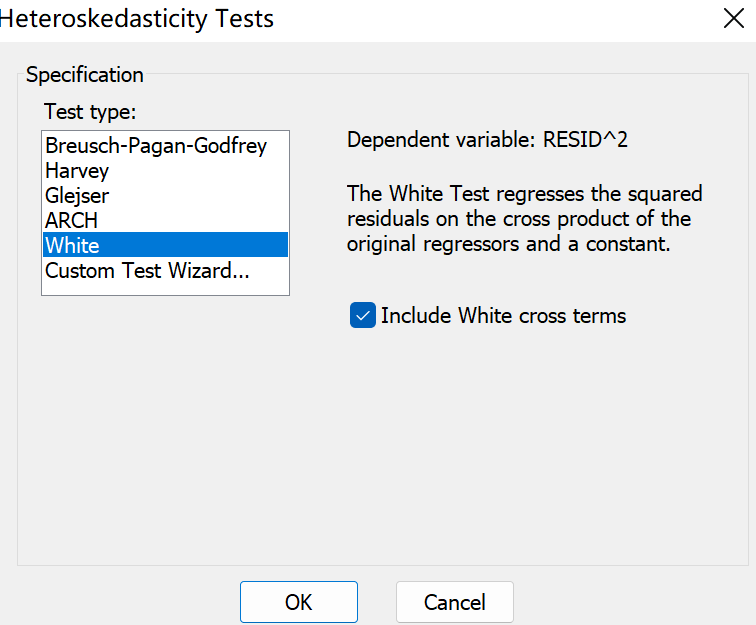
\includegraphics[width=0.55\linewidth]{figures//3回归//回归2/怀特检验的步骤.png}
    \caption{怀特检验的步骤}
    \label{怀特检验的步骤}
\end{figure}

怀特检验的结果如图\ref{怀特检验的结果}所示。

\begin{figure}[H]
    \centering
    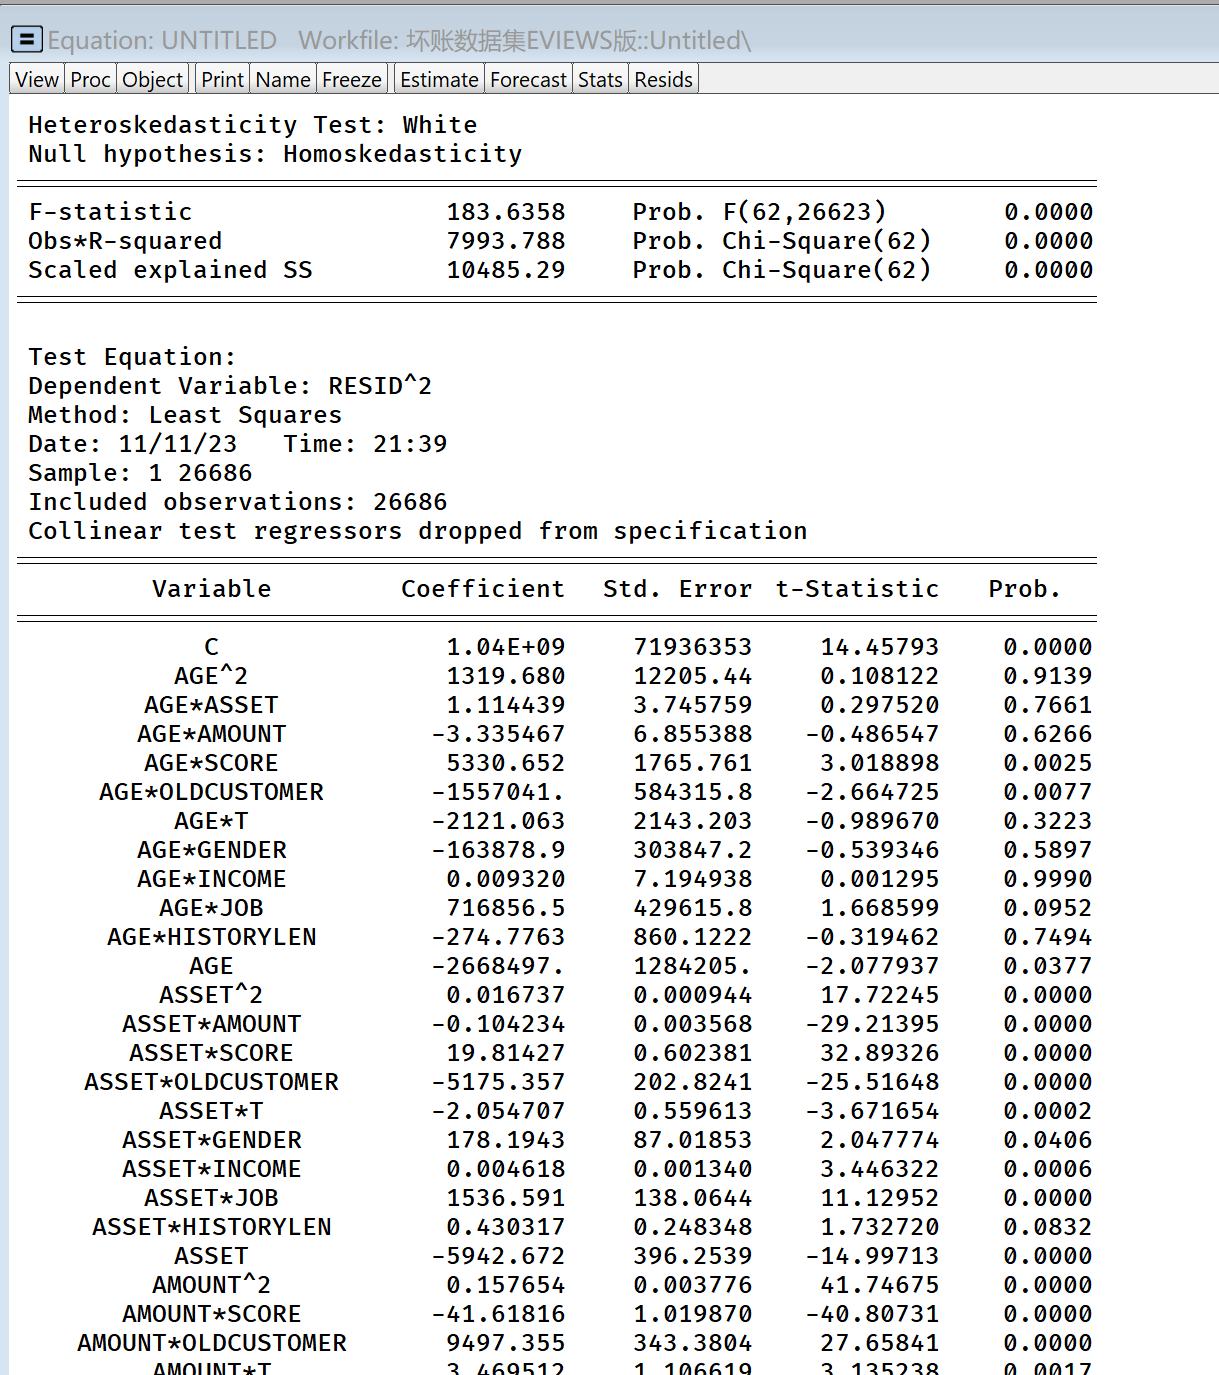
\includegraphics[width=1\linewidth]{figures//3回归//回归2/怀特检验的结果.png}
    \caption{怀特检验的结果}
    \label{怀特检验的结果}
\end{figure}

从结果可知,$nR^2$的结果为7993.788,p值>5\%,因此拒绝原假设,因此,可以得出结论——\textbf{该模型存在异方差}。


\subsubsection{模型修正}

下面,根据我们的诊断结果,我们对模型II进行进一步的调整和修正。

首先,需要删除冗余变量\texttt{gender}、\texttt{income}、\texttt{historylen};其次,对于异方差性,基于文献,我们首先尝试使用经济理论意义更强的变量\textt{lvt}代替\texttt{asset}、\texttt{amount},来消除贷款金额的增加引发的规模效应导致的异方差。\textt{lvt}的经济理论意义已经在第一部分讲述。

在Eviews中输入指令\texttt{LS baddebt c age ltv score oldcustomer t income job}进行修正回归。回归结果为——

\begin{figure}[H]
    \centering
    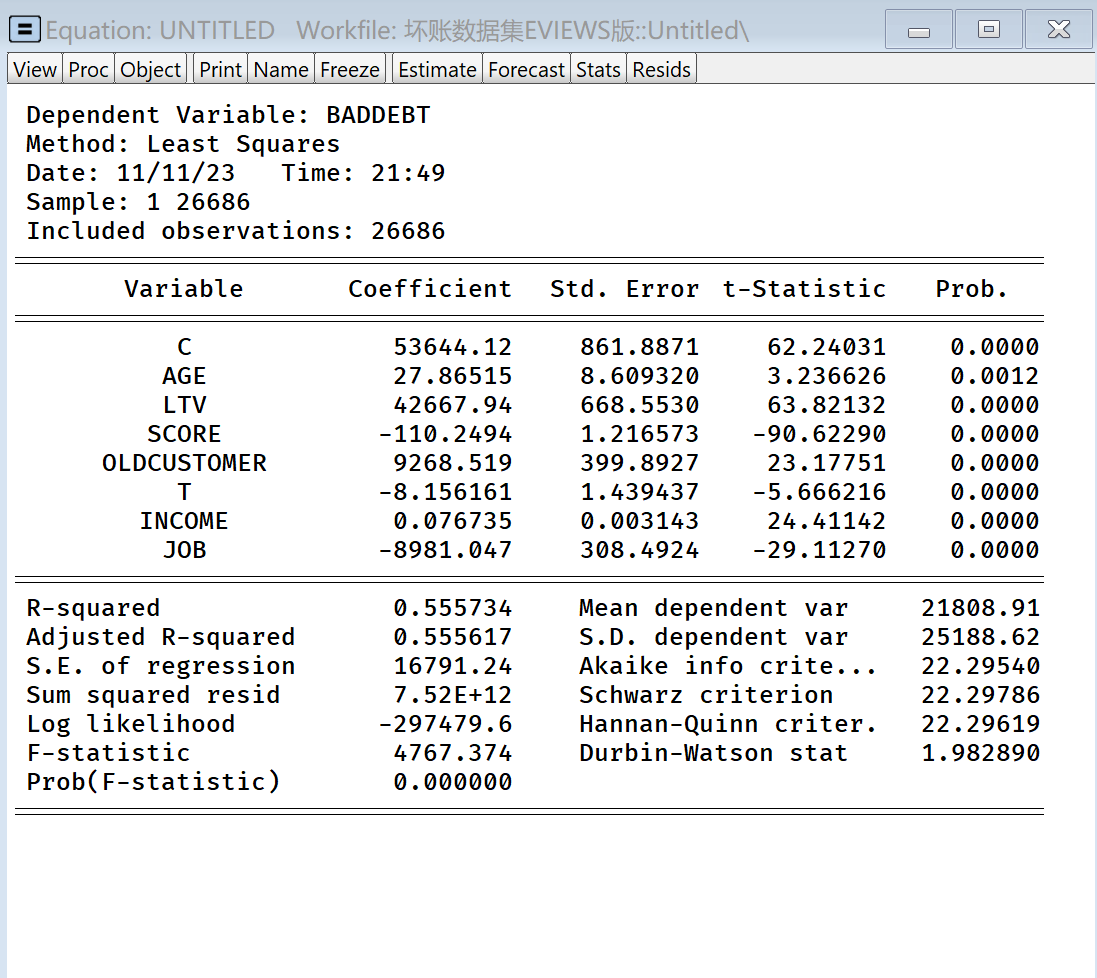
\includegraphics[width=1\linewidth]{figures//3回归//回归2/模型II修正结果.png}
    \caption{模型II修正结果(第一次)}
    \label{模型II修正结果}
\end{figure}

可以看到,所有变量均呈现较强的显著性。这意味着这些变量在所研究的模型中具有较高的影响力,对模型结果的解释具有重要意义。下面我们仍然使用white检验对模型的异方差性进行修正后的检验。检验结果如图\ref{white检验修正2-1}所示。

\begin{figure}[H]
    \centering
    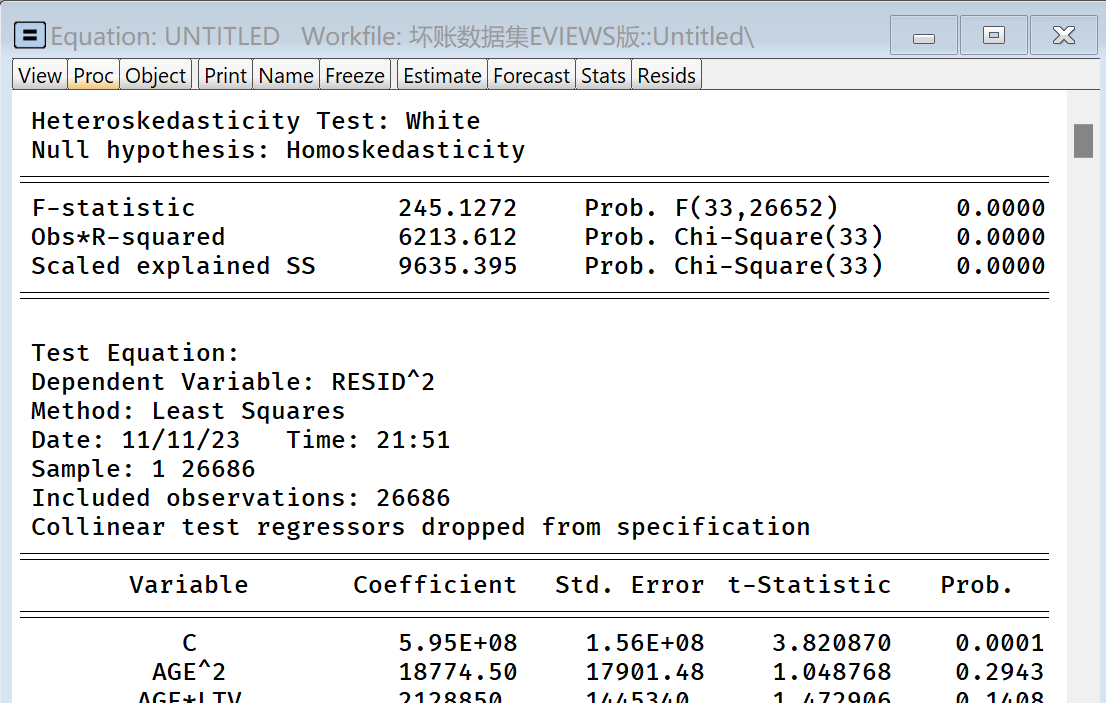
\includegraphics[width=0.75\linewidth]{figures//3回归//回归2/white检验修正.png}
    \caption{white检验第一次修正后的模型II结果}
    \label{white检验修正2-1}
\end{figure}

很遗憾,仍然存在异方差性,究其原因是\texttt{lvt}在一定程度上仍然反应了借款金额大小。但是相比之前的模型,$nR^2$值有所下降。

由于方程仍然存在异方差性,我们使用white调整的方法进行调整。通过依次点击 Estimate -> Options -> Huber-white 进行校正。

\begin{figure}[H]
    \centering
    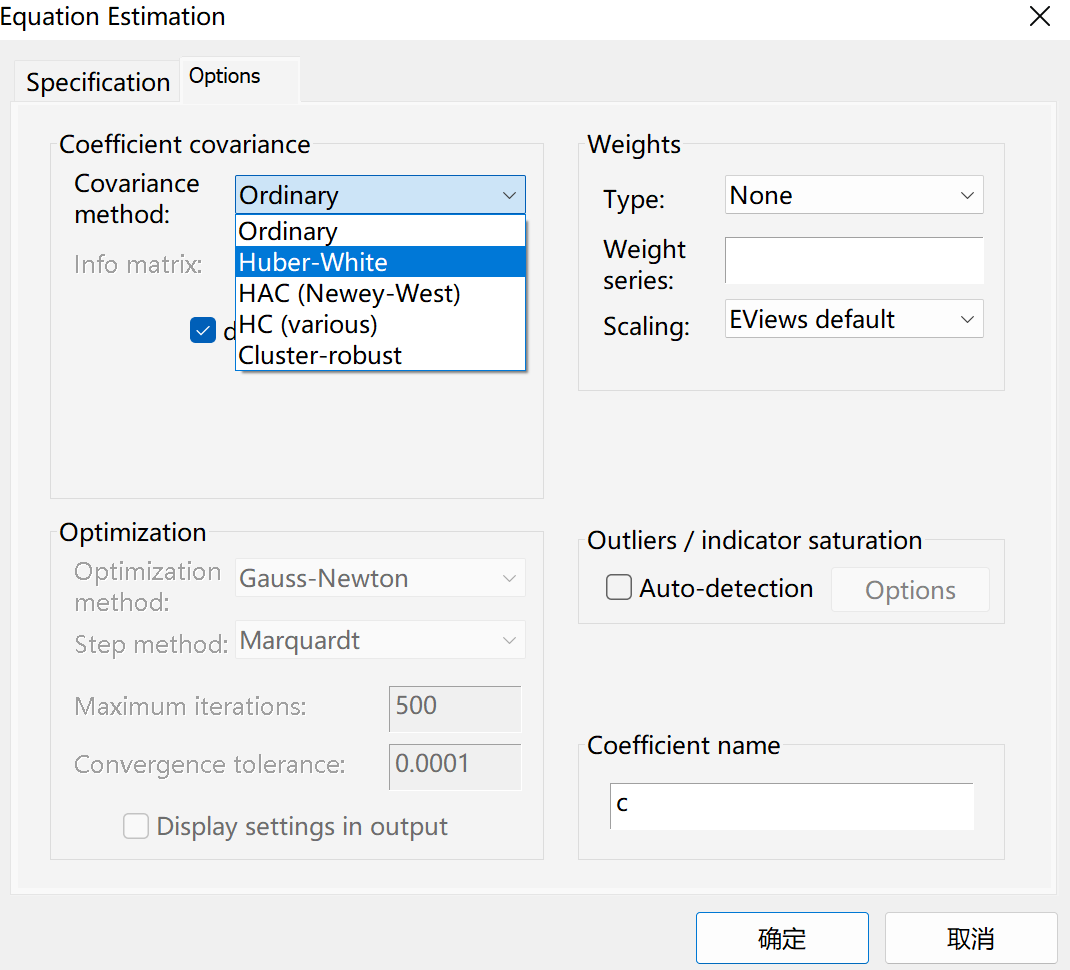
\includegraphics[width=0.5\linewidth]{figures//3回归//回归2/white调整步骤.png}
    \caption{white调整步骤}
    \label{white调整步骤}
\end{figure}

调整后的结果如图\ref{white调整后的结果}所示

\begin{figure}[H]
    \centering
    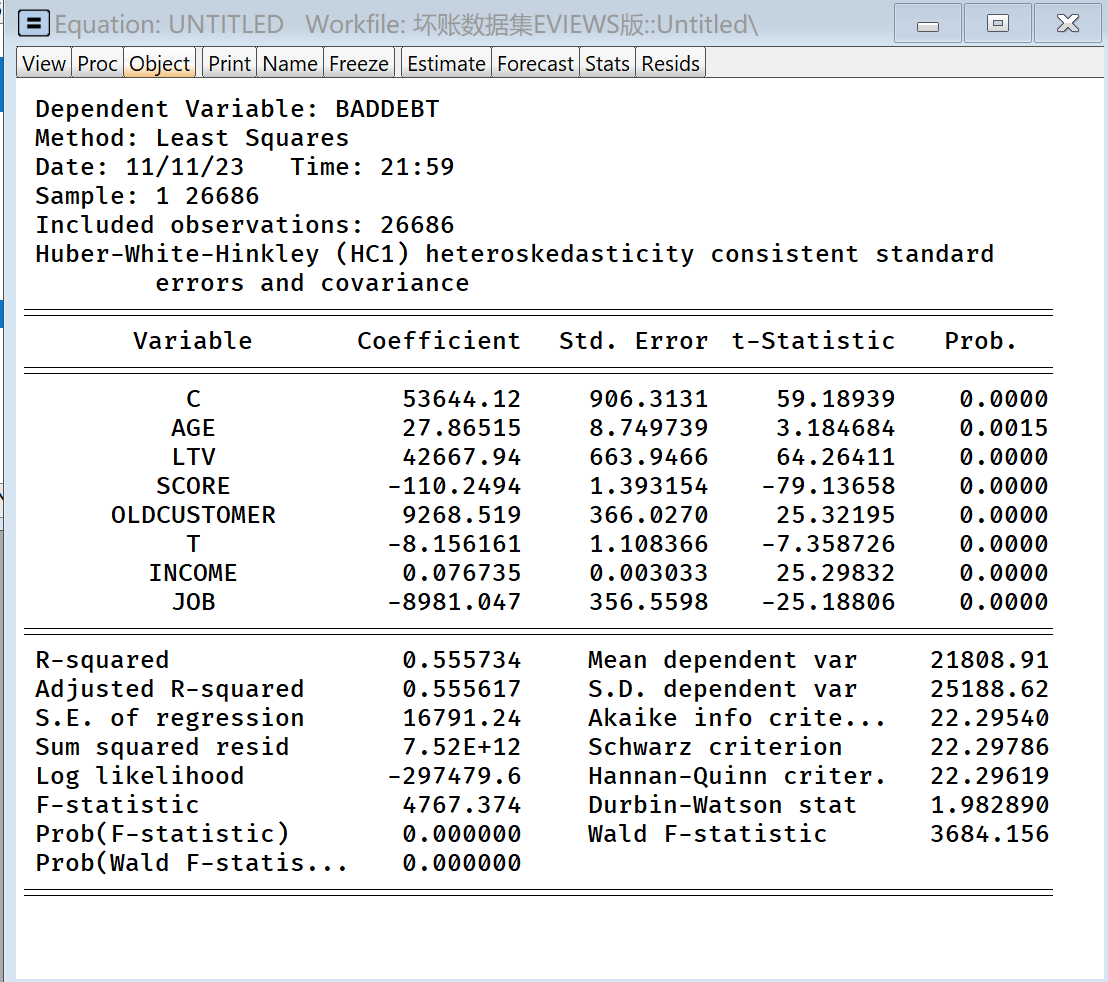
\includegraphics[width=1\linewidth]{figures//3回归//回归2/white修正后的结果.png}
    \caption{white调整后的结果}
    \label{white调整后的结果}
\end{figure}

可以看到,white调整只修正了标准误,对各个参数的系数没有改变。

最终的模型调整为

\begin{equation}
\begin{split}
 BADDEBT &= 53644.12 + 27.87\times AGE + 42667.94\times LTV \\ & - 110.25\times SCORE + 9268.52\times OLDCUSTOMER - 8.16\times T \\ & + 0.0767\times INCOME - 8981.05\times JOB
\end{split}
\end{equation}





\newpage
\section{结果分析与解释}
基于第三节对两个模型的回归结果,本节主要聚焦在模型结果的分析解释上,我们将深入分析并解释这两个模型的结果,以期更好地理解自变量与因变量之间的关系和经济意义。从而让其指导实际生活。
\subsection{模型I:还款能力模型}

根据我们在第三节所得到的回归结果,我们得到了这一样一个还款能力的Logit模型。\textbf{请注意,被解释变量取值为1时表明该借款者在借款期间存在还款困难。}

\begin{equation}
    \begin{split}
        \widehat{L:Pr(TARGET_i=1)}=&-0.70 - 0.01\times AGE - 0.14\times CAR \\ &  + 0.03\times CHILDREN + 0.22\times GEND \\ & - 0.30\times GRADUATE - 0.10\times MARRY - 0.28\times RICH \\ &  + 0.19\times POVERTY - 0.01\times ITA \nonumber
    \end{split}
\end{equation}

如表\ref{三类评价用户还款能力的影响因素},我们可以将评价用户还款能力的影响因素大致分为三类。
% Please add the following required packages to your document preamble:
% \usepackage{booktabs}
\begin{table}[H]
\setlength{\belowcaptionskip}{0.2cm}
\centering
\caption{三类评价用户还款能力的影响因素}
\label{三类评价用户还款能力的影响因素}
\begin{tabular}{c|c|c}
\hline
\textbf{个人信息} & \textbf{资产情况}  &\textbf{ 外部环境}    \\ \hline
年龄   & 是否有车  & 城市GDP评级 \\
性别   & 收入债务比 &         \\
教育水平 &       &         \\
婚姻情况 &       &         \\
子女个数 &       &         \\ \hline
\end{tabular}
\end{table}

可以看到,有关个人信息的变量占到了总变量个数的62.5\%,这表明我们在衡量一个人是否具备还款能力时,主要考究其个人与家庭的基本信息,这是因为这些信息能够很好的反映出借款人的信用状况、消费习惯和生活稳定性而具有独立的个体差异。当然,我们也会同时参考其资产情况和外部环境因素,这两者也是很重要的因素。

值得我们注意的是,对于我们之前无法预测符号的变量\texttt{graduate},其实际符号为负。其\textbf{系数的经济意义是:在保持其他变量不变的前提下,拥有更高的学历比低学历人群拥有还款困难情况的概率低7.5\%}(-0.3\times 0.5 \times 0.5=0.075)。也就是说,高学历的人往往比低学历的人信用更好。

这也符合我们的常识,在一般银行,学历更高者往往也会拥有更高的信用额度。根据\cite{基于借款人学历视角的实证检验(高学历抑制还款欠款)}的研究显示,高学历人群的收入水平较高,这使得他们在还款方面有更强的能力和稳定性。收入越高,还款压力相对较小,违约的可能性就越低;同时,高学历人群往往具备较强的信用意识,明白信用对于个人和社会的重要性。因此,他们在借款时会更加谨慎,还款时也会更加遵守承诺,降低逾期和违约行为的发生。当然,高学历人群在财务规划方面通常具备较强的能力。他们可以更好地管理个人财务,合理安排贷款还款,从而降低还款逾期及违约的风险。因此,学历之于信用是个不错的隐形“度量衡”。

我们也注意到,收入债务比这一个新引入的变量表现出较好的解释效力。其经济意义是:\textbf{在其他变量保持不变的情况下,收入债务比每增加1个单位,这个借款者拥有还款困难情况的概率就会降低2.5}\%。这启示我们,了解自己的收入债务比非常重要。这有助于他们更加清晰地认识到自己的财务状况,从而做出更为明智的消费和投资决策。在一定程度上,降低债务水平、优化负债结构,有助于提高还款能力,降低信用风险。

\subsection{模型II:坏账金额模型}

基于在第三节的结果,我们得到了这样一个估计坏账金额的线性模型。

\begin{equation}
\begin{split}
 BADDEBT &= 53644.12 + 27.87\times AGE + 42667.94\times LTV \\ & - 110.25\times SCORE + 9268.52\times OLDCUSTOMER - 8.16\times T \\ & + 0.0767\times INCOME - 8981.05\times JOB \nonumber
\end{split}
\end{equation}


上述包含了多个影响因素,如借款人的年龄、贷款价值比率(债务资产比)、信用评分、是否为老客户、贷款期限、收入和是否在职。下面就几个典型的系数分析。

首先,模型中的系数代表了各个变量对坏账金额的影响程度。从这个模型中,我们可以看出年龄、贷款价值比率、信用评分、是否为老客户、贷款期限、收入和职业这七个因素都对坏账金额有显著影响。


贷款价值比率(债务资产比)为 42667.94,这意味着\textbf{在其他条件不变的情况下,债务资产比每增加一个单位,坏账金额就有可能增加42667.94}。因此,借款人在申请贷款时,应合理评估自己的债务承受能力,避免过度负债。借款人应根据自身的收入、支出、还款能力等因素,合理规划贷款金额,以降低违约风险。

信用评分为 -110.25,表明信用评分越高,坏账金额越低。这一现象符合生活实际,因为信用评分是对借款人信用状况的一种量化衡量,评分越高,说明借款人的信用状况越好,违约风险越小。基于评分卡的贷款审批模型目前也在各大银行、信用贷款APP问世,如蚂蚁信用分、微信支付分等也已经有了成熟的评分体系。

是否为老客户的系数为 9268.52,表示老客户的坏账金额要低于非老客户。这个系数的大小超出我们的逾期。但通过分析,我们认为,银行在与老客户长期合作的过程中,积累了丰富的信用数据,可以更准确地评估老客户的信用状况。这有助于银行更加了解老客户的风险特征,从而有针对性地制定风险控制措施,降低坏账风险;同时,银行为了维护老客户关系,通常会为他们提供一定的优惠政策,如更低的利率、更高的额度等。这些政策有助于降低老客户的贷款成本,减轻还款压力,从而降低违约风险。这也就造成了老客户的坏账金额较少的缘故,\textbf{因此银行也乐意挽留老客户,而对于新客户的审查更加苛刻}。

这个模型的主要用途是预测坏账金额。通过对借款人的年龄、贷款价值比率、信用评分、是否为老客户、贷款期限、收入和职业等因素进行评估,可以预测出借款人的坏账风险,从而为金融机构提供风险管理的依据。



\newpage
\section{结论、感悟与展望}
\subsection{结论与展望}

信用贷款的审核、评估、预测一直以来都是一个复杂的难题。本文基于某公司的两个公开数据集,通过计量经济学方法回归拟合出了还款能力模型以及坏账金额预测模型。

在还款能力模型中,我们考虑了多个影响因素,如申请人的年龄、性别、婚姻状况、子女个数、教育程度、所在城市GDP评级等。通过对这些变量进行回归分析,我们得出了对应的系数,从而可以根据申请人的信息预测其还款能力。这一模型有助于贷款机构在审核贷款申请时,更加准确地评估申请人的信用风险。

坏账金额预测模型则针对已经发生违约的贷款,通过分析违约贷款的债务资产比、信用评级、年龄等因素,拟合出了一个预测模型。该模型可以预测出贷款发生违约时的坏账金额,为贷款机构在发生坏账时提供了一定的防范和应对措施。

通过建立这两个模型对于信贷机构开展信贷业务具有重要作用,其一方面可以消除高风险借款人减少个人消费信贷违约风险,其另一方面可以寻找“高质量”的信贷人,实现双赢局面。在未来,这种应用将进一步发挥其潜力,为信贷市场带来更多积极影响。相信随着大数据和人工智能技术的发展,模型的设定和调整会更加精确,信贷机构能更全面地了解借款人的信用状况,提高贷款审核的精准度。

\subsection{感想与感悟}

本次计量经济学小组作业由小组三名同学齐心完成,第一节由***负责编写,第二节由***负责编写,第四节由***负责编写,第三节由三人共同完成。在完成本次作业的过程中,收获颇多。

首先,我们对计量经济学的方法有了更深入的理解和掌握。通过本次小组作业,我们对回归分析、预测模型等方法的应用有了更为直观的认识,明白了如何将理论知识运用到实际问题中。

其次,我们在数据处理和分析方面积累了宝贵的经验。在完成作业的过程中,我们学会了如何使用统计软件进行数据处理,如何从数据集中提取有用信息,以及如何基于模型存在的问题进行诊断、修正、弥补。这些经验将在未来的学术研究和实际工作中发挥重要作用。

此外,本次作业使我们认识到团队合作的重要性。在小组讨论和分工合作的过程中,我们学会了如何有效沟通、如何协调不同观点,以及如何高效完成任务。这种团队协作能力对于我们未来的学术和职业生涯都具有深远影响。

同时,本次作业也让我们意识到计量经济学在实际问题中的应用价值。通过构建还款能力模型和坏账金额预测模型,我们发现计量经济学方法可以帮助信贷机构更好地评估借款人的信用风险,从而降低违约风险。这使我们更加坚定了将理论知识与实际问题相结合的决心。

最后,本次作业使我们认识到自身在知识体系和技能方面的不足。在完成作业的过程中,我们发现自己在某些方面的理论知识尚不完善,对某些实际问题的理解仍有待提高。这激发了我们在今后的学习中更加努力,不断提升自己的综合素质。

总之,本次计量经济学小组作业为我们带来了丰富的收获。我们将以此为契机,继续深入学习和探索计量经济学领域,为未来的学术和职业生涯打下坚实基础。




%%----------- 参考文献 -------------------%%
%在reference.bib文件中填写参考文献,此处自动生成
\newpage
\reference

\thispagestyle{empty} % 首页不显示页码
\addcontentsline{toc}{section}{参考文献}\tolerance=500 %将参考文献放进目录
\end{document}